\chapter{MATERIAL PROPUESTO}

\begin{center}
	\textbf{PREGUNTAS TEÓRICAS}
	\\
	
\end{center}

\begin{enumerate}
	%%%%%%%%%%%%%%%%%%%%%%1
	\item~ Responda breve y claramente   los siguientes enunciados:
	\begin{enumerate}
		\item Especifique la clasificación de las estaciones de radiodifusión de FM de acuerdo a su potencia de transmisión.
		\item Compare dos de los sistemas de modulación estudiados, enunciando dos ventajas y dos desventajas.
		\item Elabore una tabla comparativa con tres (3) parámetros establecidos en Colombia para los sistemas de radiodifusión AM y FM.
		\item Explique en qué consiste el efecto umbral.
		\item Explique brevemente qué es preénfasis y deénfasis
		\item Explique y dé un ejemplo de la representación fasorial de señales moduladas en onda continua.
		\item Explique brevemente qué es heterodino
		\item Describa la importancia de la coherencia en la detección de señales moduladas linealmente.
		
		\item~ Enuncie dos (2) diferencias fundamentales entre la modulación AM y la modulación FM.
		\item~ Defina proceso aleatorio.
	\end{enumerate}


%%%%%%%%%%%%%%%%%%%%%%2

\item~ El Plan Técnico Nacional de Radiodifusión Sonora (PTNRS) en Frecuencia Modulada  define diferentes clases de estaciones de radio FM según su potencia de transmisión (potencia radiada aparente, p.~r.~a.) así:

\begin{itemize}
	\item \textbf{ESTACIÓN CLASE A}: Mínimo 15 kW y máximo 100 kW de p. r. a., en la dirección de máxima ganancia de la antena.
	\item \textbf{ESTACIÓN CLASE B}: Superior a 5 kW e inferior a 15 kW de p. r. a., en la dirección de máxima ganancia de la antena.
	\item \textbf{ESTACIÓN CLASE C}: Superior a 250 W y máximo 5 kW de p. r. a., en la dirección de máxima ganancia de la antena.
	\item \textbf{ESTACIÓN CLASE D}: Máximo 250 vatios de p. r. a., en la dirección de máxima ganancia de antena.
\end{itemize}

También se define el \textbf{PORCENTAJE DE MODULACIÓN} como \textit{``la razón de la oscilación real de la frecuencia a la oscilación de frecuencia definida como el 100\% de modulación a una oscilación de frecuencia de $\pm75$~kHz"} (Tenga en cuenta que en FM, porcentaje de modulación e índice de modulación son dos parámetros distintos`, ya que el porcentaje de modulación corresponde a la desviación de frecuencia real comparada con la máxima autorizada).

Adicionalmente, establece que 
``\textit{Cuando para la prestación del servicio de radiodifusión sonora, se requiera frecuencia de enlace entre los estudios y el sistema de transmisión, ésta hará parte integrante de la concesión y los derechos por su uso se cancelarán de acuerdo con el reglamento respectivo}".

De acuerdo al PTNRS, a la emisora UIS Estéreo ``La Voz de la Universidad", que tiene asignado el distintivo HKW23, le corresponde la frecuencia 96,9~MHz, con potencia de transmisión de 10~kW y frecuencia de enlace entre los estudios y el sistema de transmisión de 328,5~MHz. Los estudios de la emisora están ubicados en la sede UIS Bucarica, a 4,3~km (LOS) del sistema de transmisión, que se encuentra en el Alto de los Padres. 

Con base en lo anterior y respecto a la emisora UIS Estéreo:
\begin{enumerate}
	\item Determine a qué clase de estación corresponde.
	\item Identifique con qué frecuencia de portadora se emite la señal FM desde los estudios hacia el sistema de transmisión.
	
	
	\item Identifique con qué frecuencia de portadora se emite la señal FM desde el sistema de transmisión.
	
	
	\item Dibuje el espectro de potencia (en dB) de la señal emitida por el sistema de transmisión si la portadora no está modulada.
	
	
	\item Calcule el porcentaje de modulación cuando se alcanza una desviación de frecuencia de 50~kHz.
	
	\item Dibuje el espectro de potencia (en dB) de la señal emitida por el sistema de transmisión si la portadora está modulada al 100\% por un tono de frecuencia 15 kHz.
	
	
	\item Dibuje un diagrama de bloques del sistema de transmisión, asumiendo que la potencia que recibe este sistema proveniente de los estudios es de 0 dB. 
\end{enumerate}
%%%%%%%%%%%%%%%%%%%%
\item~ En el plan técnico nacional de radiodifusión sonora en frecuencia modulada, se define emisión fuera de banda como: 

\textit{``Emisión en una o varias frecuencias situadas fuera de la anchura de banda necesaria, cuyo nivel puede reducirse sin influir en la transmisión de la información correspondiente. Las emisiones armónicas, las emisiones parásitas, los productos de intermodulación y los productos de conversión de frecuencia, están comprendidas en las emisiones no esenciales, pero están excluidas de las emisiones fuera de banda"}.

Además el plan establece que: 
\textit{``Las emisiones no esenciales, con respecto a la portadora sin modular, deben atenuarse de la siguiente manera:}

\begin{tabular}{ll}
	\textbf{Separación con la portadora} & \textbf{Atenuación} \\
	Entre 120 y 240 kHz. & 25 dB \\
	Entre 240 y 600 kHz. & 35 dB
\end{tabular}

\textit{Para separaciones de más de $600$~kHz con respecto a la portadora, se debe aplicar el valor que resulte de la expresión:}
\begin{center}
	Atenuación $A[$dB$] = 43 + 10 \log (P[$W$])$,
\end{center}
siendo $P$ la potencia de transmisión de la señal.

Teniendo en cuenta lo anterior, si se tiene una señal FM de una estación clase D con frecuencia de portadora 90~MHz y 200~W de potencia:

\begin{enumerate}
	\item Dibuje la magnitud (en dB) de la respuesta en frecuencia de un filtro ideal que garantice el cumplimiento de la norma en relación con las emisiones no esenciales.
	
	\item Explique si la porción de densidad espectral de potencia de emisiones no esenciales que se muestra en la siguiente figura cumple o no la normatividad respectiva.

\vspace{100px}
%\setcounter{figure}{130}
\begin{figure}[h!]
	\captionsetup{justification = raggedright, singlelinecheck = false}
	\caption{Ejercicio tres} 
	\centering
	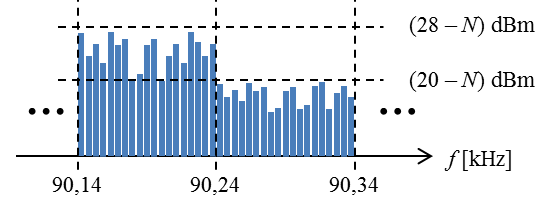
\includegraphics[scale=1]{Imagenes/fig01.png}
	\label{fig:fig01}
	%	\captionsetup{justification=raggedright,font={scriptsize,bf,it}}
	%	\caption*{fuente: llllll}
\end{figure}

\item Según la norma citada, explique con sus palabras la diferencia entre emisiones no esenciales y emisiones fuera de banda.
	\end{enumerate}
%%%%%%%%%%%%%%%%%%%4
\item~ En el Plan Técnico Nacional de Radiodifusión Sonora en Amplitud Modulada, numeral 3.1.2, se define \textbf{anchura de banda necesaria} como:

\textit{``Anchura de la banda de frecuencias estrictamente suficiente para asegurar la transmisión de información con la velocidad y calidad requerida y en condiciones específicas."}

y en el numeral 3.1.6, se define \textbf{emisión fuera de banda }como: 

\textit{``Emisión en una o varias frecuencias situadas fuera de la anchura de banda necesaria, cuyo nivel puede atenuarse sin influir en la transmisión de la información correspondiente. Las emisiones armónicas, las emisiones parásitas, los productos de intermodulación y los productos de conversión de frecuencia, están comprendidas en las emisiones no esenciales, pero están excluidas de las emisiones fuera de banda."}

Tanto las emisiones fuera de banda, como las emisiones no esenciales de las que habla esta definición, son consideradas \textit{emisiones no deseadas}.

Además el plan establece que: 
\textit{``Las emisiones no esenciales, con respecto a la portadora sin modular, deben atenuarse:}

\begin{center}
	\begin{tabular}{ll}
		De 10 a 20 kHz: & -25 dB \\ 
		De 20 a 30 kHz: & -35 dB \\
		De 30 a 75 kHz: & -35 dB menos 1 dB/kHz
	\end{tabular}
\end{center}

\textit{De 75 kHz en adelante así: para transmisores con potencia hasta de 5~kW: -80~dB. Para transmisores con potencias superiores a 5~kW se debe aplicar el valor que resulte de aplicar la expresión:}
\begin{center}
	Atenuación $A[$dB$] = 43 + 10 \log (P[$W$])$,
\end{center}
siendo $P$ la potencia de la portadora sin modular.

Teniendo en cuenta lo anterior, si se tiene una señal AM de una estación con potencia de portadora de 4~kW y frecuencia $890$~kHz, dibuje la magnitud (en dB) de la respuesta en frecuencia de un filtro que garantice el cumplimiento de la norma en relación con las emisiones no esenciales.
%%%%%%%%%%%%%%%%%5
\item~Subraye UNA posible respuesta de las que aparecen en paréntesis para obtener un enunciado verdadero, y encierre en un círculo el numeral que corresponda a una justificación apropiada para el siguiente enunciado:

En el Plan Técnico Nacional de Radiodifusiòn Sonora en Frecuencia Modulada se definen:

\textit{\textbf{PREÉNFASIS}: Incremento del nivel de altas frecuencias de audio en proporción directa al aumento de amplitud del ruido en dichas frecuencias, antes de la modulación, con el fin de mantener una relación constante a través de toda la banda de transmisión.}

\textit{\textbf{DEÉNFASIS}: Procedimiento para reducir la amplitud de las frecuencias altas después de su detección en los receptores, con el fin de restituir el nivel relativo original de la banda de transmisión.}\\

Con base en lo anterior se puede afirmar que un sistema preénfasis-deénfasis en FM (\textbf{incrementa/
	disminuye}) la relación señal a ruido en la (\textbf{transmisión/recepción}) debido a que:
\begin{enumerate}
	\item contrarresta el comportamiento cuadrático del ruido.
	\item minimiza las causas del efecto umbral.	
	\item mejora el ancho de banda efectivo de la señal recibida.
\end{enumerate}
\end{enumerate}

\pagebreak
\begin{center}
\textbf{MODULACIÓN DE ONDA CONTINUA}
\\

\end{center}
\begin{enumerate}

\item~ Considere el sistema de modulación mostrado en la siguiente figura, donde $m_v(t)$ es una señal de video monocromático con ancho de banda cercano a los 4,2~MHz que se modula linealmente con portadora $f_{cv}$, $m_a(t)$ es una señal de audio que se modula angularmente con portadora $f_{ca}=f_{cv}+4,5$~MHz, el Filtro 1 tiene frecuencia central $f_{1}=f_{cv}+2,5$~MHz, y el Filtro 2 tiene frecuencia central $f_{2}=f_{ca}$.\\


\begin{figure}[h!]
	\captionsetup{justification = raggedright, singlelinecheck = false}
	\caption{Ejemplo sistema de modulación} 
	\centering
	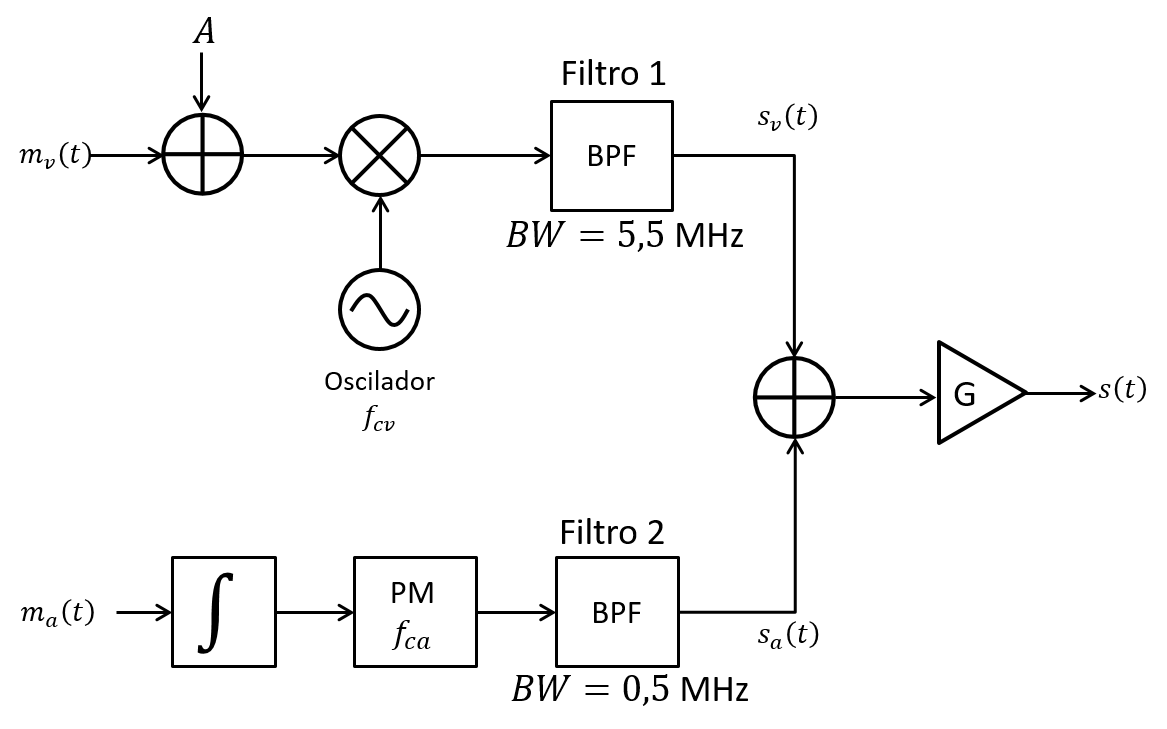
\includegraphics[scale=0.5]{Imagenes/ntscdiagram.png}
	\label{fig:ntscdiagram}
	%	\captionsetup{justification=raggedright,font={scriptsize,bf,it}}
	%	\caption*{fuente: llllll}
\end{figure}

%\begin{center}
%	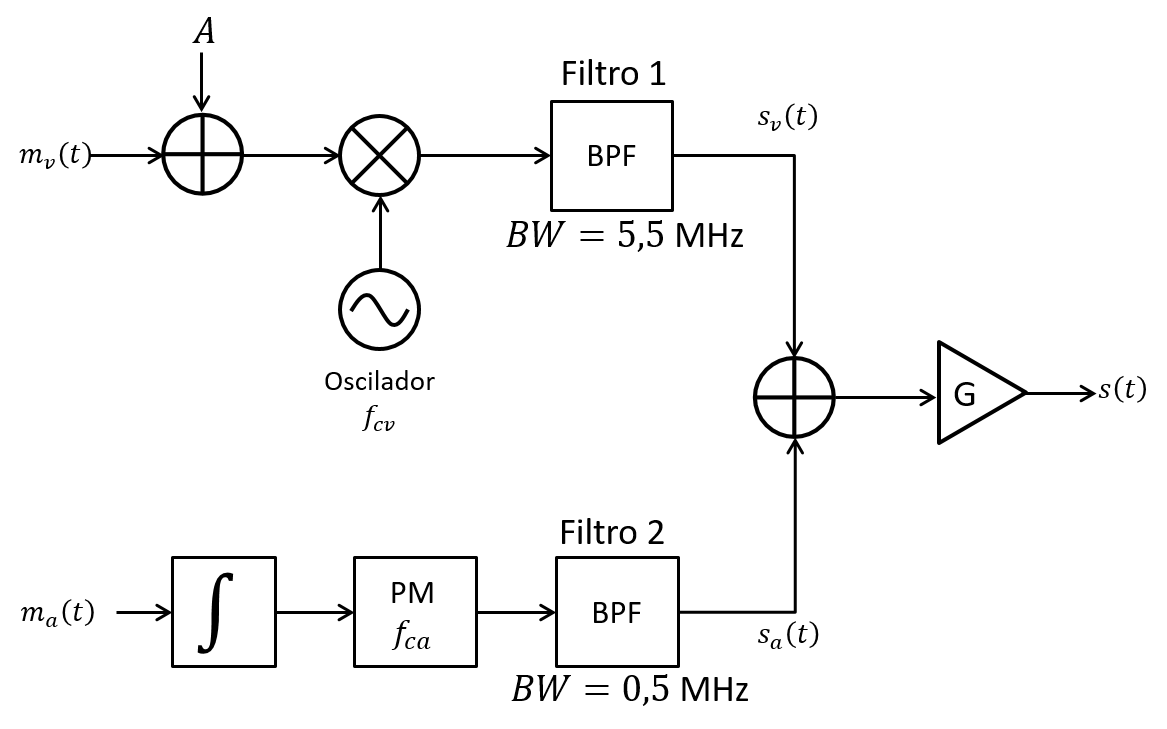
\includegraphics[scale=0.5]{imagenes/ntscdiagram.png} 
%\end{center}
Asumiendo que $A\gg m_v(t)$ y que $f_{cv}$ es mucho mayor que el ancho de banda de las señales de entrada:
\begin{enumerate}
	\item Determine el tipo de modulación de $s_v(t)$.
	
	\item Determine el tipo de modulación de $s_a(t)$.
	\item Esboce el espectro de la señal transmitida $s(t)$.
	
	\item ¿Qué clase de multiplexión se realiza con $s_v(t)$ y $s_a(t)$ para obtener $s(t)$? 
	
	\item ¿Qué clase de demodulador emplearía para recuperar $s_v(t)$ y por qué?
	
	
	\item ¿Qué justifica no emplear la misma clase de modulador para las señales $m_v(t)$ y $m_a(t)$?		
\end{enumerate}

%%%%%%%%%%%2
\item~ Se tiene un modulador FM de banda ancha como se muestra en la siguiente figura (asuma que el mezclador incluye su propio filtro pasabandas):


%\begin{center}
%	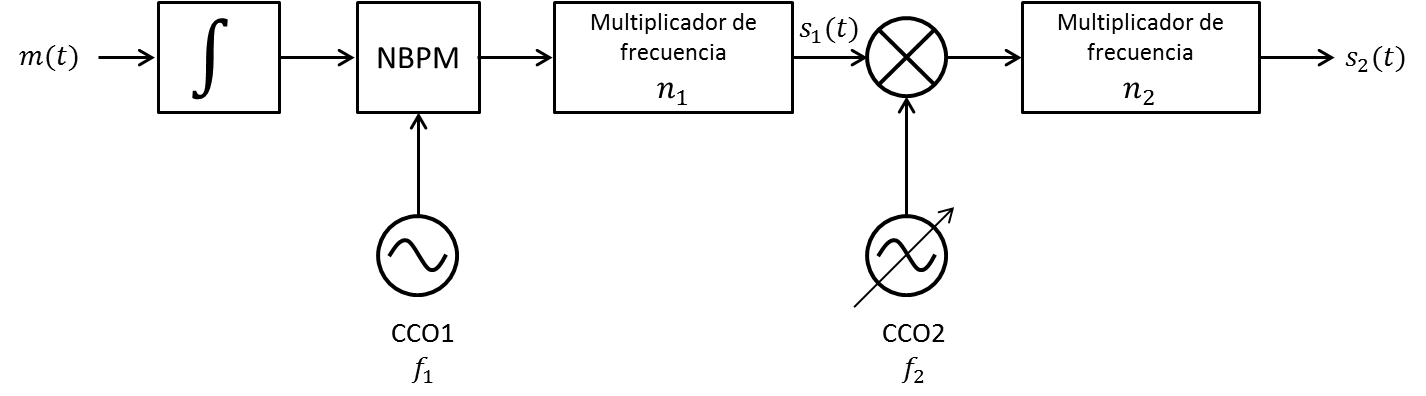
\includegraphics[scale=0.7]{imagenes/fig1.png} 
%\end{center}

\vspace{200px}
\begin{figure}[h!]
	\captionsetup{justification = raggedright, singlelinecheck = false}
	\caption{Ejemplo modulador FM} 
	\centering
	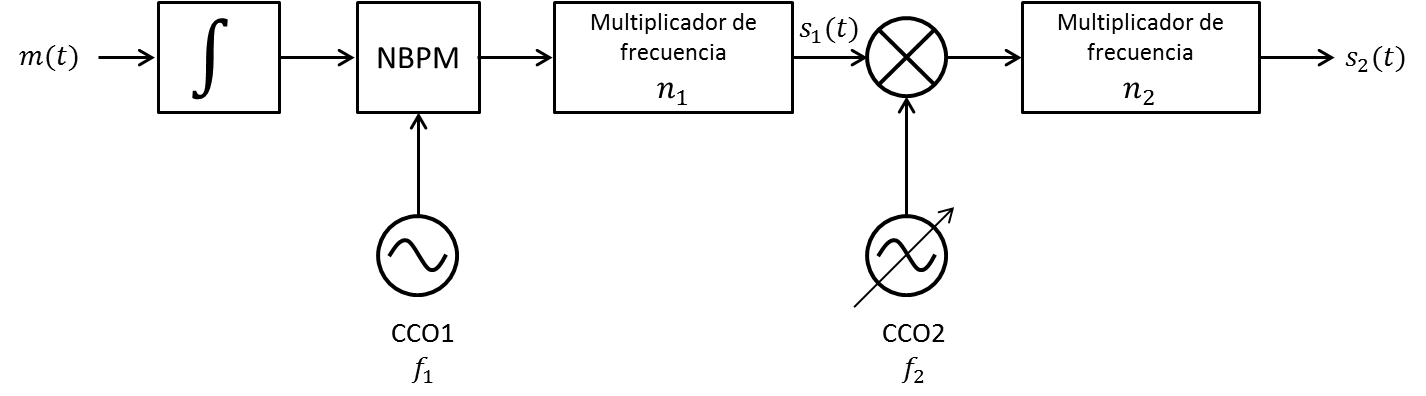
\includegraphics[scale=0.7]{Imagenes/fig1.png}
	\label{fig:fig1}
	%	\captionsetup{justification=raggedright,font={scriptsize,bf,it}}
	%	\caption*{fuente: llllll}
\end{figure}

donde los CCO corresponden a osciladores controlados por cristal, y el bloque NBPM es un modulador PM de banda estrecha con coeficiente de sensibilidad $k_p$~[rad/V]. \\

Este modulador es utilizado para transmitir señales de audio $m(t)$ en el rango de frecuencias entre 100 Hz y 15 kHz. La frecuencia del primer oscilador es tal que $f_1 \le 1$~MHz. La máxima desviación de frecuencia de la señal $s_2(t)$ es de 75~kHz y la señal $s_1(t)$ debe tener frecuencia de portadora $f_{c1} = 10,7$~MHz. 

De acuerdo a lo anterior:

\begin{enumerate}
	\item Determine una expresión analítica para $s_2(t)$ en términos de los parámetros del sistema.
	
	\item Estime por dos métodos diferentes el ancho de banda de la señal $s_2(t)$ si la entrada es un tono de frecuencia 15~kHz.
	
	\item Encuentre valores para los parámetros del sistema tal que la señal de salida tenga frecuencia de portadora $f_{c2} = 90$~MHz~$\pm$~2 kHz, e indique el valor de desviación de frecuencia de la señal $s_1(t)$.
	
	\item Asuma que se requiere que el CCO2 sea un oscilador de frecuencia variable tal que $s_2(t)$ pueda generarse a cualquier frecuencia de portadora del rango de frecuencias comerciales de radio FM en Colombia. 
	\begin{enumerate}
		\item ¿Cómo se verían afectadas las diferentes etapas de diseño del literal anterior?
		
		
		\item ¿Cómo debería variar la frecuencia $f_2$?
	\end{enumerate}
\end{enumerate}
%%%3
\item~ Se tiene una señal FM, $s(t)$, modulada por un tono $V_m(t)=10\sin(2\pi 2000t)$~[V], con índice de modulación $\beta=1$. Si la portadora no modulada es $V_c (t)=10\cos(2\pi 2\times 10^5 t)$~[V]:
\begin{enumerate}
	\item~ Dibuje la densidad espectral de potencia de la señal (en dBm) asumiendo una resistencia de carga de $50~\Omega$.
	\item~ Determine el ancho de banda de la señal empleando dos métodos diferentes.
	
	\item~ Diseñe un modulador que satisfaga las condiciones dadas por el enunciado, a partir de un VCO de frecuencia de libre oscilación $f_o=40$~kHz, y coeficiente de sensibilidad $k_f=2$~[V$^{-1}$], como se muestra en la figura:
%	\begin{center}
%		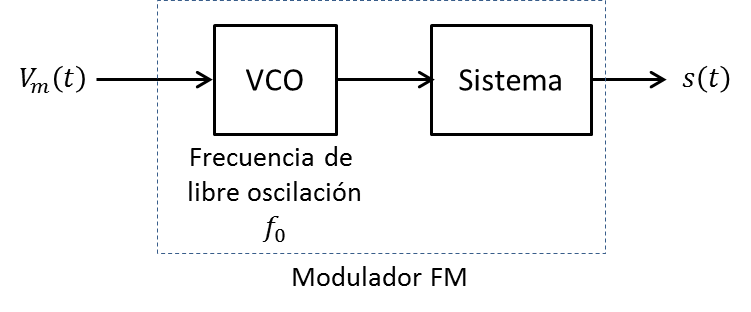
\includegraphics[scale=0.65]{imagenes/fig002.png} 
%	\end{center}

\vspace{200px}

\begin{figure}[h!]
	\captionsetup{justification = raggedright, singlelinecheck = false}
	\caption{Modulador FM} 
	\centering
	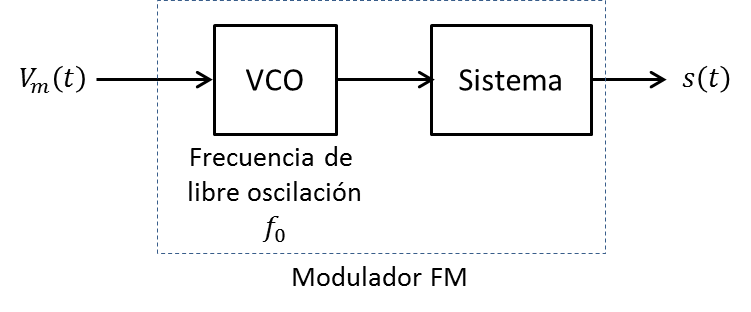
\includegraphics[scale=0.65]{Imagenes/fig002.png}
	\label{fig:fig002}
	%	\captionsetup{justification=raggedright,font={scriptsize,bf,it}}
	%	\caption*{fuente: llllll}
\end{figure}
	
\end{enumerate}
%%%%%%%%%%%%%%%%%%4
\item~Considere una señal FM $s(t)=A_c \cos[2\pi f_c t + 2\pi k_f\int{m(\tau)d\tau}]$ modulada por un tono $m(t)=A_m \cos(2\pi f_m t)$, con frecuencia de portadora $f_c=104,5$ MHz, cuya densidad espectral de potecia se observa en un analizador de espectros, tal como se muestra en la siguiente figura:

%\vspace{100px}
\begin{figure}[h!]
	\captionsetup{justification = raggedright, singlelinecheck = false}
	\caption{Imagen analizador de espectro} 
	\centering
	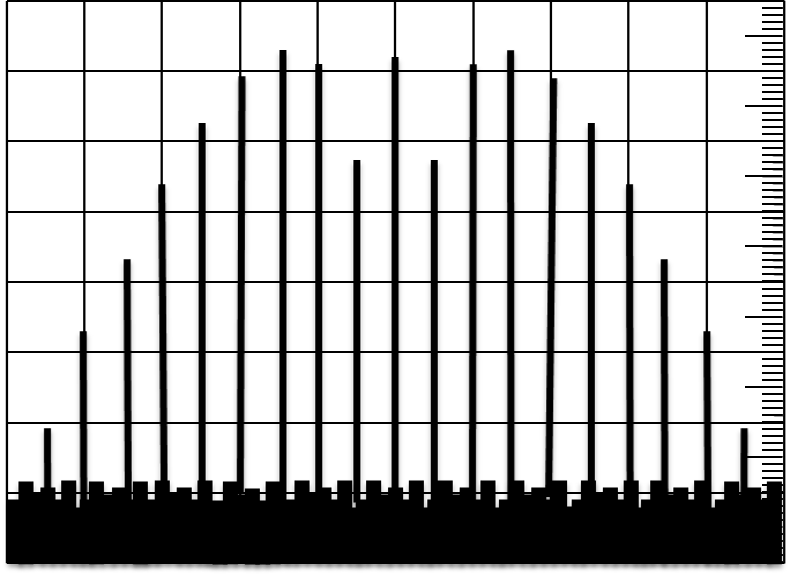
\includegraphics[scale=0.42]{Imagenes/Espectro.png}
	\label{fig:EEspectro}
	%	\captionsetup{justification=raggedright,font={scriptsize,bf,it}}
	%	\caption*{fuente: llllll}
\end{figure}
%\begin{center}
%	\includegraphics[scale=0.42]{imagenes/espectro.png} 
%\end{center}

\begin{itemize}
	\item Nivel de referencia: 1 dBm
	\item Escala vertical: 10 dB/div
	\item Frecuencia central: 104,5 MHz
	\item SPAN: 10 kHz/div
\end{itemize}

\begin{enumerate}
	\item Determine la potencia $P_T$ total de la señal modulada (en [dBm]).
	\item Estime la potencia de la portadora SIN modular $P_c $  (en [dBm]).
	\item Determine la frecuencia del mensaje $f_m$  (en [Hz]).
	\item Estime el índice de modulación de $s(t)$ Y $\beta$.
	\item Determine el ancho de banda $B_T$ de la señal modulada, especificando claramente el criterio utilizado. 
	
\end{enumerate}

%%%%%%%%%%%%%%%%5
\item~Considere el siguiente esquema de modulación lineal: 
%\begin{center}
%	\includegraphics[scale=0.42]{imagenes/esquema.png} 
%\end{center}	

\vspace{200px}
\begin{figure}[h!]
	\captionsetup{justification = raggedright, singlelinecheck = false}
	\caption{Sistema de modulación lineal} 
	\centering
	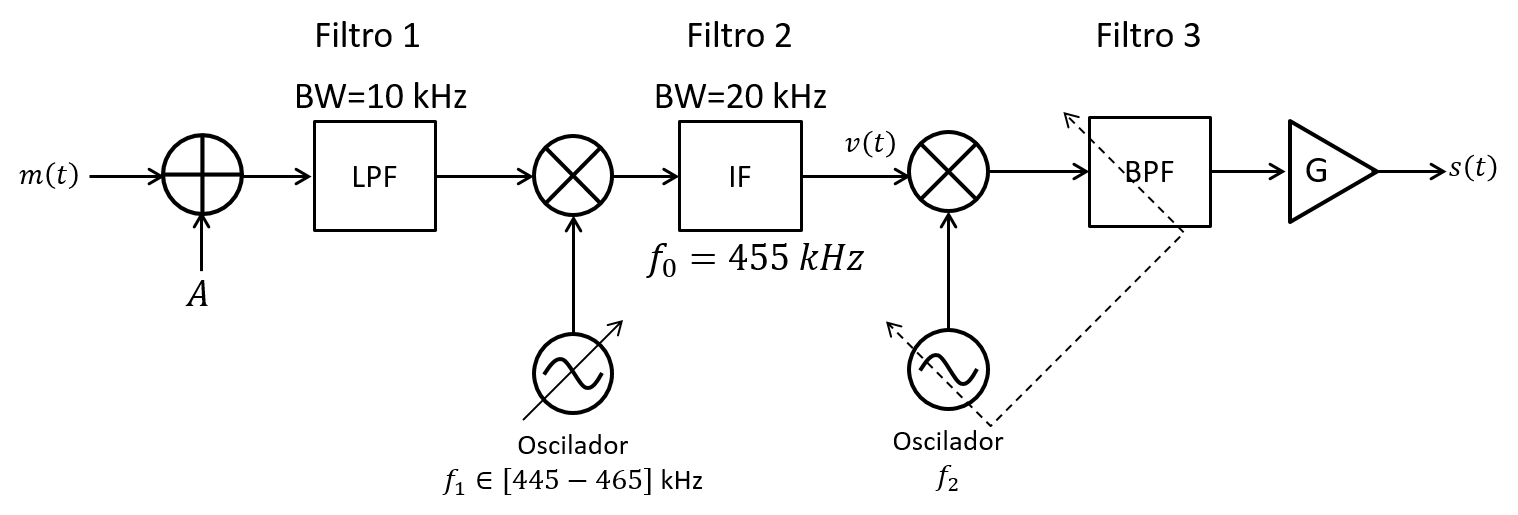
\includegraphics[scale=0.42]{Imagenes/Esquema1.png}
	\label{fig:Esquema1}
	%	\captionsetup{justification=raggedright,font={scriptsize,bf,it}}
	%	\caption*{fuente: llllll}
\end{figure}

donde $m(t)$ es una señal mensaje de media cero, los filtros son ideales de ganancia unitaria, al igual que la amplitud de los osciladores, y el amplificador tiene una ganancia $G=40$ dB.

\begin{enumerate}
	\item Determine a qué clase de señal modulada corresponde $v(t)$ si:
	\begin{center}
		\begin{tabular}{|c|c|c|}
			\hline
			$A$ & $f_1$ & Tipo de modulación \\ \hline
			1 & 445 kHz & \rule[1mm]{0mm}{5mm}\\ \hline 
			1 & 455 kHz & \rule[1mm]{0mm}{5mm} \\ \hline
			0 & 455 kHz & \rule[1mm]{0mm}{5mm} \\ \hline
			0 & 465 kHz & \rule[1mm]{0mm}{5mm} \\ \hline
		\end{tabular}
	\end{center}
	
	\item ¿En qué rango de frecuencias debe variar $f_2$ con el fin de poder obtener una señal AM con una frecuencia de portadora que se pueda escoger entre 540 y 1700 kHz?
	
	\item Si $m(t)=\cos(10000\pi t)$, y se desea obtener una señal AM a la salida con porcentaje de modulación del 100\% y frecuencia de portadora de $(900)$~kHz:
	\begin{itemize}
		\item Encuentre los valores de $A$, $f_1$, y $f_2$. 
		\item Asumiendo que la frecuencia central del Filtro 3 es $(900)$~kHz, determine el mínimo y el máximo ancho de banda posibles para este filtro.
		\item Calcule la potencia  $P_T=$ de la señal $s(t)$ en[dBm]
		\item Grafique $s(t)$ vs $m(t)$.
		
	\end{itemize}
	
	\item ¿Qué consideraciones se deben tener en cuenta al diseñar el Filtro 3?
\end{enumerate}

%%%%%%%%%6
\item~ Considere el siguiente esquema de modulación y demodulación:
%\begin{center}
%	\includegraphics[scale=0.7]{imagenes/ESQUEMA2.png} 
%\end{center}	

\vspace{400px}
\begin{figure}[h!]
	\captionsetup{justification = raggedright, singlelinecheck = false}
	\caption{Esquema de modulación y demodulación.} 
	\centering
	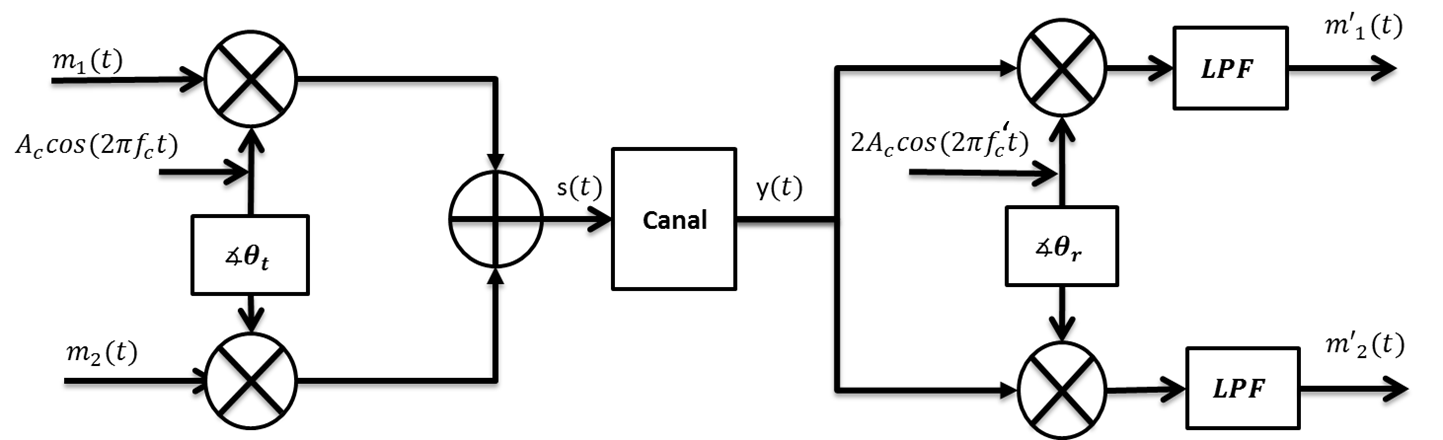
\includegraphics[scale=0.6]{Imagenes/Esquema2.png}
	\label{fig:Esquema2}
	%	\captionsetup{justification=raggedright,font={scriptsize,bf,it}}
	%	\caption*{fuente: llllll}
\end{figure}

tal que $\theta_t=\pi/2$, y los mensajes $m_1(t)$ y $m_2(t)$ tienen un ancho de banda $B << f_c$. Asumiendo un canal ideal:

\begin{enumerate}
	\item ¿Qué clase de modulación se obtiene con este sistema? 
	
	\item ¿Qué clase de modulación se obtiene con este sistema si $m_1(t)=m_2(t)$? Encuentre una expresión de $s(t)$ que justifique su respuesta. 
	
	\item Asumiendo que $\theta_r = \theta_t$, y si $f_c^\prime =f_c+\Delta f$, encuentre: $m_1'(t)$, $m_2'(t)$. Compare el efecto cuando $\Delta f << B$ y $\Delta f >> B$. 
	
	\item Asumiendo que $f_c^\prime = f_c$, y si $\theta_r = \theta_t+\Delta \theta$,  encuentre: $m_1'(t)$), $m_2'(t)$. Describa el efecto del error de fase $\Delta \theta$ en la demodulación.
	
	
	¿Qué valor(es) de $\Delta \theta \in (0,2\pi]$ sería(n) indeseable(s) y por qué? 
	
	\item Comparando los resultados de los dos literales anteriores, ¿cuál efecto es más indeseable? Justifique.
	
\end{enumerate}
%%%%%%%%%7
\item~ Sea una señal FM $s(t)=A_c \cos(2\pi f_c t + 2\pi k_f\int{m(\tau)d\tau})$ con portadora $c(t)=25\cos(10^5\pi t)$~[V], modulada por un mensaje $m(t)$ y coeficiente de sensibilidad $k_f=10^3$~[Hz/V]. La señal modulada $s(t)$ es enviada a través de un canal con ruido AWGN con densidad espectral de potencia $N_0/2$, siendo $N_0 = 10^{-8}$~[W/Hz].

\begin{enumerate}
	\item Si el mensaje tiene amplitud 1~V y una densidad espectral de potencia $S_M(f)$ como la mostrada en la siguiente figura, \textbf{\emph{estime}} el ancho de banda de la señal modulada: $B_T $, y calcule en [dBm] la potencia del mensaje: $P_m$. 
%	\begin{center}
%		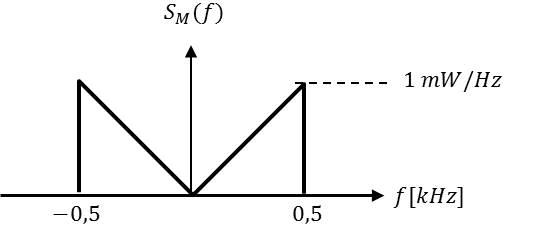
\includegraphics[scale=1]{imagenes/img0001.png} 
%	\end{center}

\begin{figure}[h!]
	\captionsetup{justification = raggedright, singlelinecheck = false}
	\caption{Densidad espectral} 
	\centering
	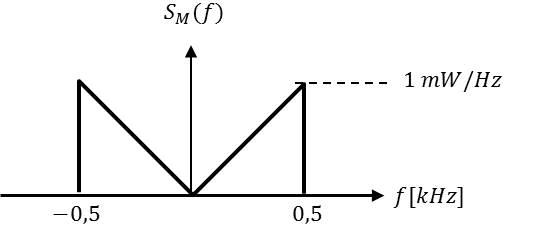
\includegraphics[scale=1]{Imagenes/img0001.png}
	\label{fig:img0001}
	%	\captionsetup{justification=raggedright,font={scriptsize,bf,it}}
	%	\caption*{fuente: llllll}
\end{figure}	
	
	\item Considerando un mensaje $m(t)=\cos(1000\pi t)$~[V], calcule el ancho de banda que contiene al menos el 75\% de la potencia total $B_T(75\%)$, y la relación señal a ruido en [dB] a la salida de un demodulador FM ideal: SNR$_O$.  
	
	\item Considerando que un mensaje $m(t)=\cos(1000\pi t)$~[V], pasa por un filtro con respuesta en frecuencia $H_P(f)$ tal que $|H_P(f)|^2=1+\left( f/f_0 \right) ^2$ \textbf{\emph{antes}} de la modulación, y que a la salida del demodulador FM ideal se incorpora un filtro con respuesta en frecuencia $H_D(f)$ tal que $|H_D(f)|^2=1/ \left(1+\left( f/f_0 \right) ^2\right)$, encuentre una expresión para la relación señal a ruido en [dB] a la salida de   este último filtro, si se sabe que $f_0=1100$ Hz. 
	
	
\end{enumerate}
%%%%%%%%%%%%%%%%8
\item~ Considere las señales $m_1(t)$ y $m_2(t)$ que se observan en las siguientes figuras.
%\begin{center}
%	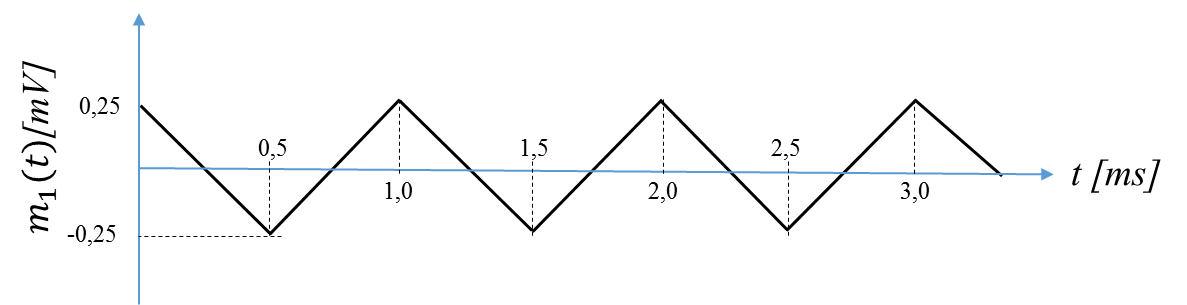
\includegraphics[scale=0.7]{imagenes/2015-1.png} 
%\end{center}

\begin{figure}[h!]
	\captionsetup{justification = raggedright, singlelinecheck = false}
	\caption{Señal $m_1(t)$} 
	\centering
	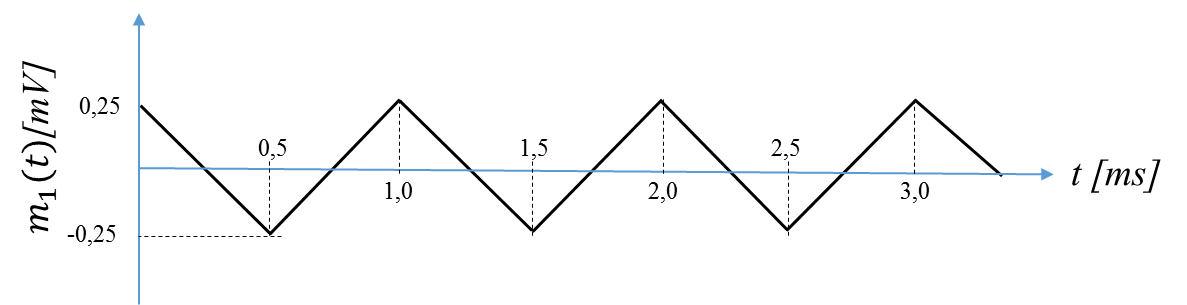
\includegraphics[scale=0.7]{Imagenes/2015-1.png}
	\label{fig:2015-1}
	%	\captionsetup{justification=raggedright,font={scriptsize,bf,it}}
	%	\caption*{fuente: llllll}
\end{figure}

\begin{figure}[h!]
	\captionsetup{justification = raggedright, singlelinecheck = false}
	\caption{Señal $m_2(t)$} 
	\centering
	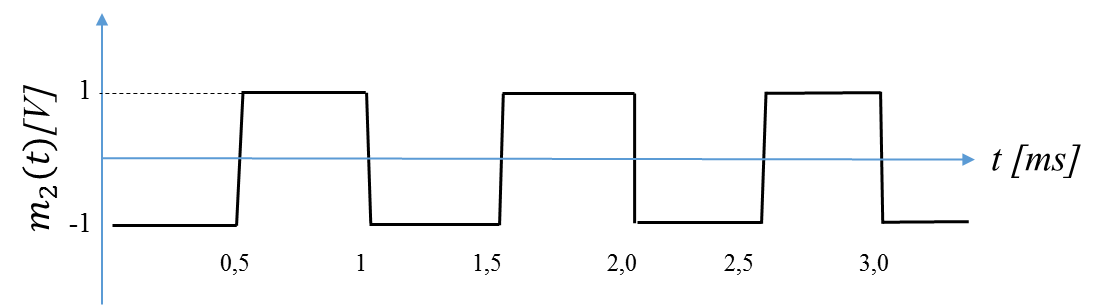
\includegraphics[scale=0.7]{Imagenes/2015-2.png}
	\label{fig:2015-2}
	%	\captionsetup{justification=raggedright,font={scriptsize,bf,it}}
	%	\caption*{fuente: llllll}
\end{figure}
%\begin{center}
%	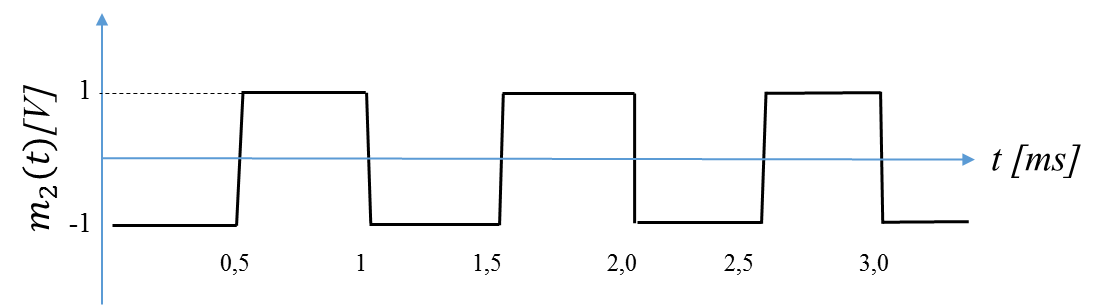
\includegraphics[scale=0.7]{imagenes/2015-2.png} 
%\end{center}
La señal $s_1(t)$ corresponde a una portadora de frecuencia $f_c$ modulada en fase por $m_1(t)$, con un coeficiente de sensibilidad $k_p=1\pi\times 10^3$~rad/V, y la señal $s_2(t)$ es una portadora también de frecuencia $f_c$ modulada en frecuencia por $m_2(t)$, con un coeficiente de sensibilidad $k_f=1$~kHz/V. Para cada señal modulada:
\begin{enumerate}
	\item Calcule la desviación de frecuencia.
	\item Estime el ancho de banda por dos métodos diferentes. ¿Se puede considerar una señal banda estrecha? Explique.
	\item Determine el coeficiente de sensibilidad tal que se obtenga una señal de ancho de banda 200~kHz aproximadamente. Compare $s_1(t)$ y $s_2(t)$.
\end{enumerate}

%%%%%%%%%%%%%%%%%%%%%%9
\item~La siguiente figura ilustra la operación de un \textit{transponder} (satélite) con frecuencia intermedia (IF) de 70 MHz. El \textit{transponder} opera en la Banda C con frecuencias para el enlace de subida (\textit{uplink}) de $[5,9 - 6,4]$~GHz ($x(t)$), y para el enlace de bajada (\textit{downlink}) de $3,7 - 4,2$~GHz ($y(t)$).

\vspace{200px}
\begin{figure}[h!]
	\captionsetup{justification = raggedright, singlelinecheck = false}
	\caption{Transponder} 
	\centering
	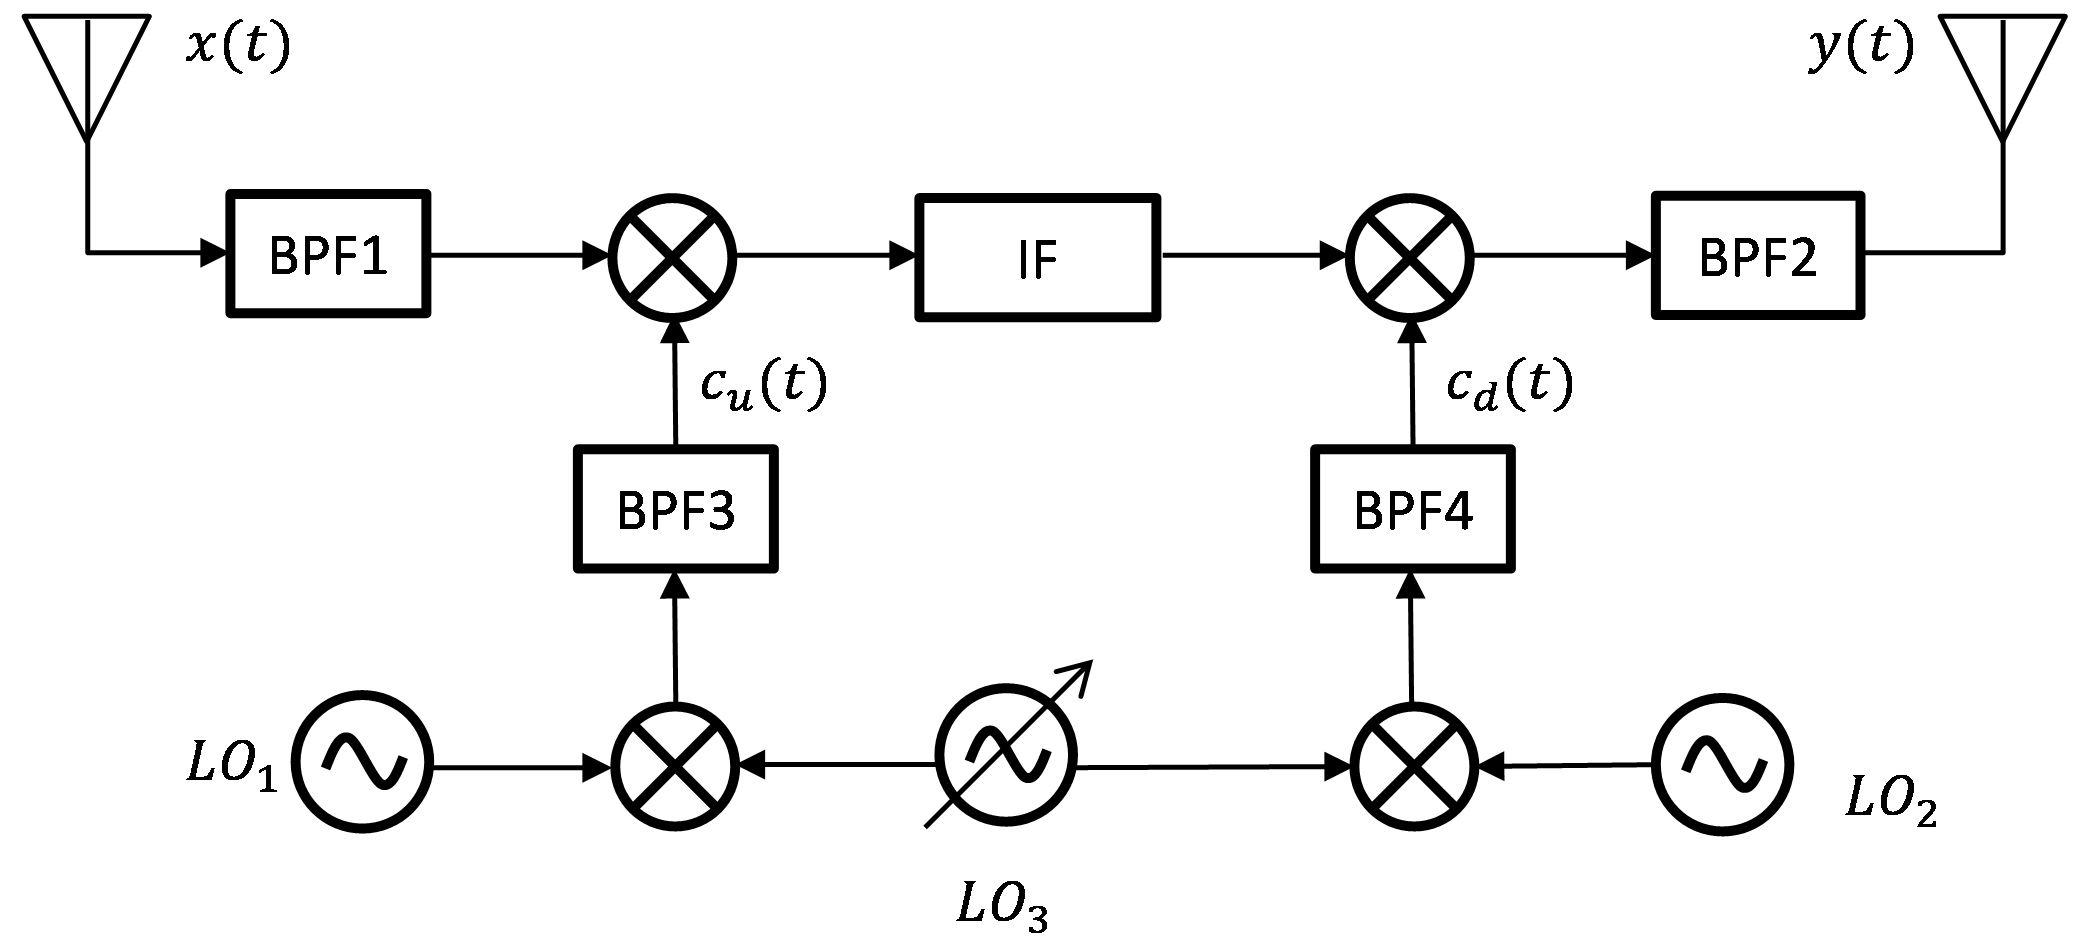
\includegraphics[scale=0.25]{Imagenes/fig4sup.png}
	\label{fig:fig4sup}
	%	\captionsetup{justification=raggedright,font={scriptsize,bf,it}}
	%	\caption*{fuente: llllll}
\end{figure}

%\begin{center}
%	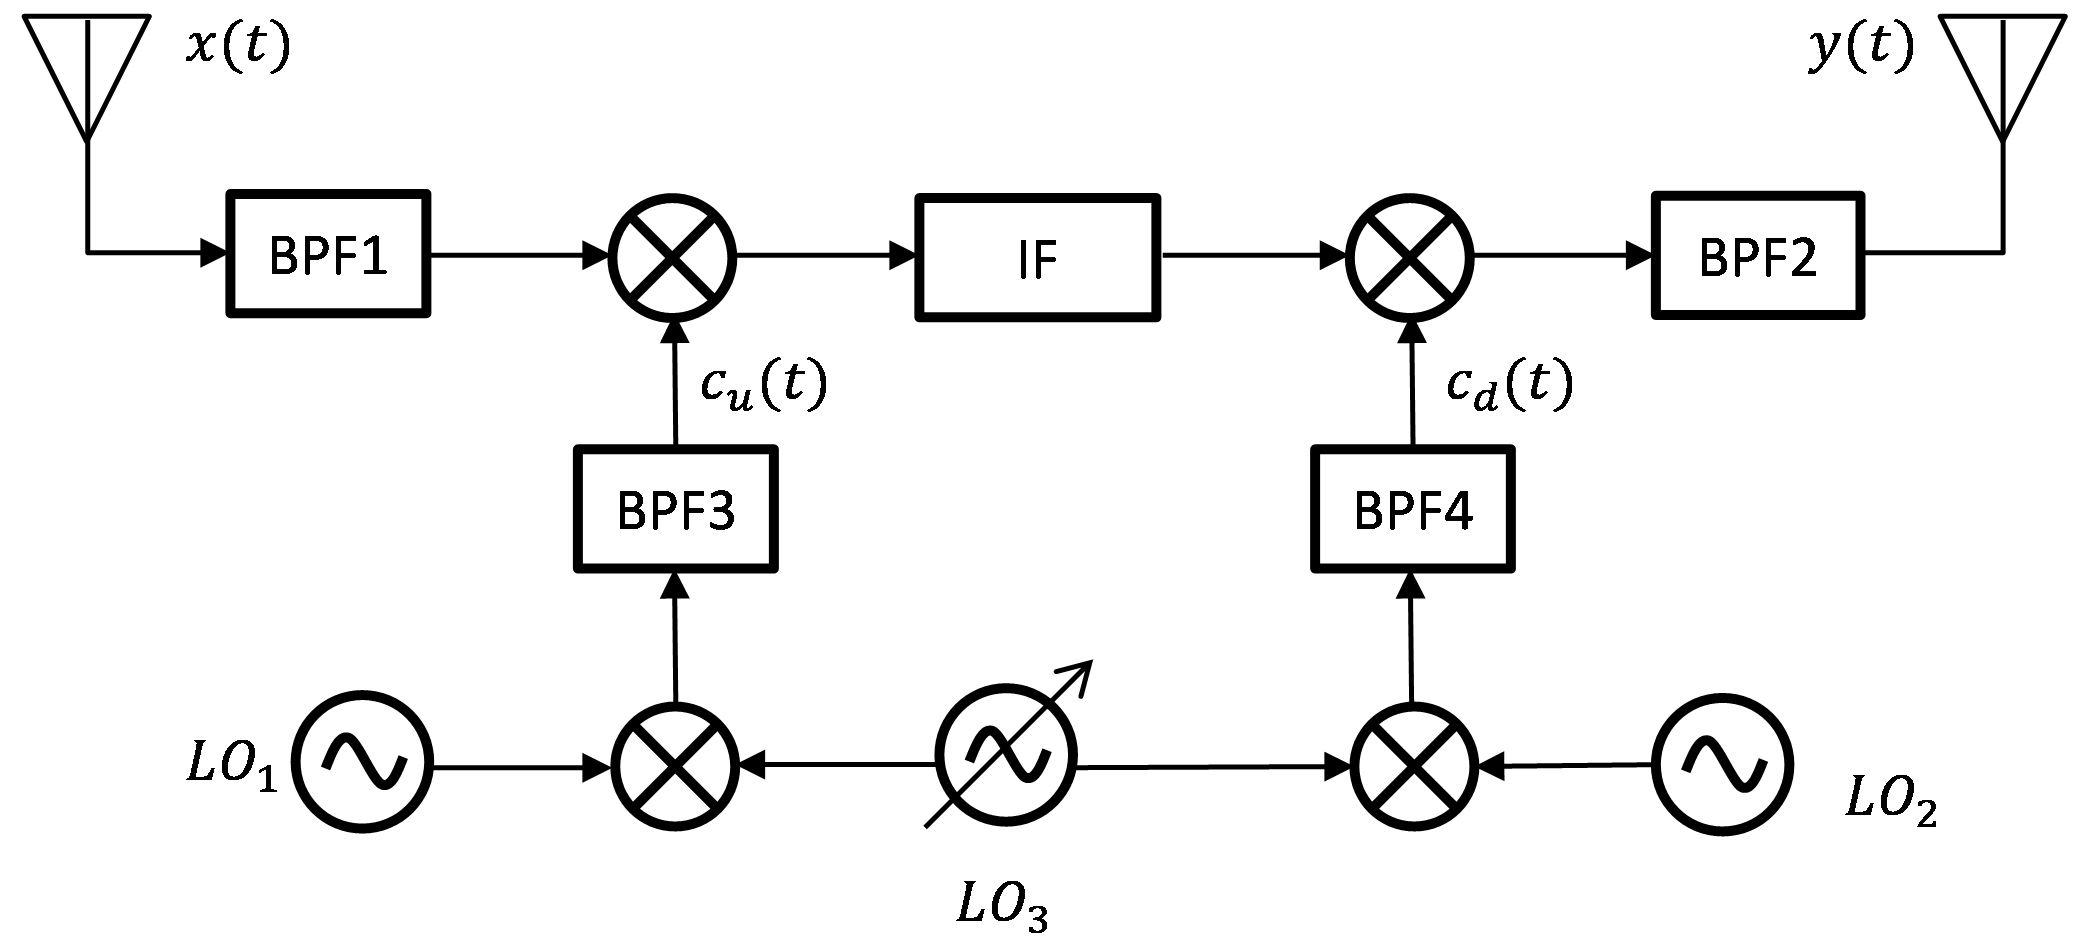
\includegraphics[scale=0.25]{imagenes/fig4sup.png} 
%\end{center}

Asumiendo que solamente el oscilador local 3 ($LO_3$) es variable, y que la señal recibida $x(t)$ tiene un ancho de banda de $30$~MHz con frecuencia de portadora dentro del rango de las frecuencias del enlace de subida:

\begin{enumerate}
	\item~ Especifique los filtros y las frecuencias de los osciladores locales del \textit{transponder} buscando reducir al máximo la frecuencia del oscilador variable $LO_3$.
	\begin{table}[h]
	\captionsetup{justification = raggedright,singlelinecheck = false}
	\caption{Ejercicio nueve.}
	\label{tabla:tabla15}
		\centering
			\scalebox{0.90}{
	\begin{tabular}{|c|c|c|c|c|c|c|c|c|}
		\hline 
		& BPF1 & BPF2 & BPF3 & BPF4 & Filtro IF & $LO_1$ & $LO_2$& $LO_3$     \\
		\hline
		Frecuencia   &   & & & &  & &  &  \qquad\qquad\qquad\qquad\qquad\qquad  \\[20pt]
		\hline
		Ancho de banda& & & & & & - & -& - \\[20pt]
		\hline
	\end{tabular}}
\end{table}
	\item~ Si la frecuencia de portadora de $x(t)$ es 6,1~GHz, y según el diseño propuesto en $(a)$, ¿cuál será la frecuencia del oscilador variable $LO_3$ y la frecuencia de portadora $f_c$ de la señal de salida $y(t)$?\\
	
	
	\item~ Analice y explique una (1) ventaja y una (1) desventaja de esta implementación respecto a otra donde $c_u(t)$ y $c_d(t)$ provengan directamente de sendos osciladores.\\
	
\end{enumerate}
%%%%%%%%%%%%%%%10
\item~ Sea la señal modulada $s(t) = A_c \cos(2\pi f_c t) + m(t)\cos(2\pi   f_c t) + \widehat{m}(t)\sin(2\pi f_c t) $, donde el mensaje $m(t)$ tiene ancho de banda 
$B= 15-N$~[kHz] y se cumple que $m(t)\ll A_c$. Esta señal se demodula mediante un detector de envolvente. 

\begin{enumerate}
	\item~ Identifique el tipo de modulación de la señal $s(t)$.
	\item~ Determine la relación señal a ruido a la entrada $SNR_I$ y salida $SNR_O$ del
	demodulador, así como la figura de mérito del mismo.($SNR_I $ , $SNR_O $,
	$\eta = $ ).
	
	\item~ ¿Qué papel juega la presencia del término $A_c \cos(2\pi f_c t)$ en la operación del sistema demodulador presentado y cómo interpreta la figura de mérito obtenida?\\
	
\end{enumerate}


%%%%%%%%%%%%%%%%%%11
\item~ Considere el siguiente sistema:

\vspace{200px}
\begin{figure}[h!]
	\captionsetup{justification = raggedright, singlelinecheck = false}
	\caption{Modulador AM} 
	\centering
	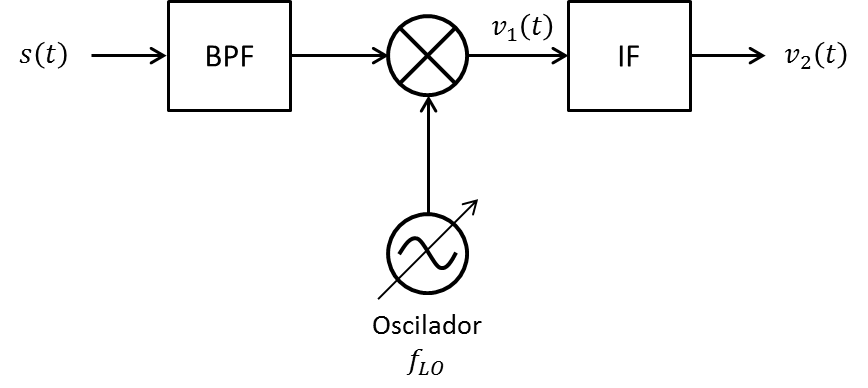
\includegraphics[scale=0.65]{Imagenes/2014.png}
	\label{fig:2014}
	%	\captionsetup{justification=raggedright,font={scriptsize,bf,it}}
	%	\caption*{fuente: llllll}
\end{figure}
%\begin{center}
%	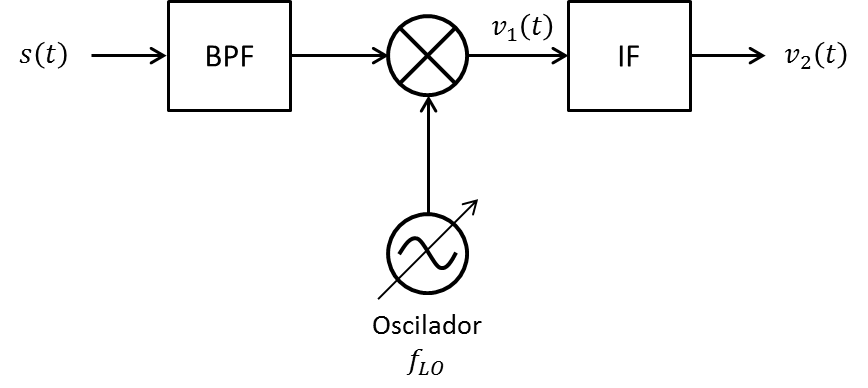
\includegraphics[scale=0.65]{imagenes/2014.png} 
%\end{center}


donde se tiene un oscilador local de frecuencia $f_{LO}$ variable. La señal $s(t)$ corresponde a una señal de \textbf{{radio AM comercial}}, cuya frecuencia de portadora está en el rango de 0,54 a 1,70 MHz. El bloque IF corresponde a un filtro pasabanda de ancho de banda 20~kHz y frecuencia central de 0,455~kHz. 
\begin{enumerate}
	\item Determine un intervalo de frecuencias en el que debería variar $f_{LO}$ con el fin de trasladar cualquiera de las posibles frecuencias de la señal $s(t)$ de entrada a la frecuencia del filtro IF. 
	\item Explique con un ejemplo la limitación de este sistema derivada de tener un filtro fijo a la entrada. 
	\item  Analice el comportamiento de la figura de mérito del sistema con entrada $s(t)$ y salida $v_2(t)$.
\end{enumerate}
%%%%%%%%%%%%%%%%%%%%%%%12

\item~ Se obtiene una señal $s(t)$ a partir de dos señales AM, como se muestra en la siguiente figura:

\begin{figure}[h!]
	\captionsetup{justification = raggedright, singlelinecheck = false}
	\caption{Modulador} 
	\centering
	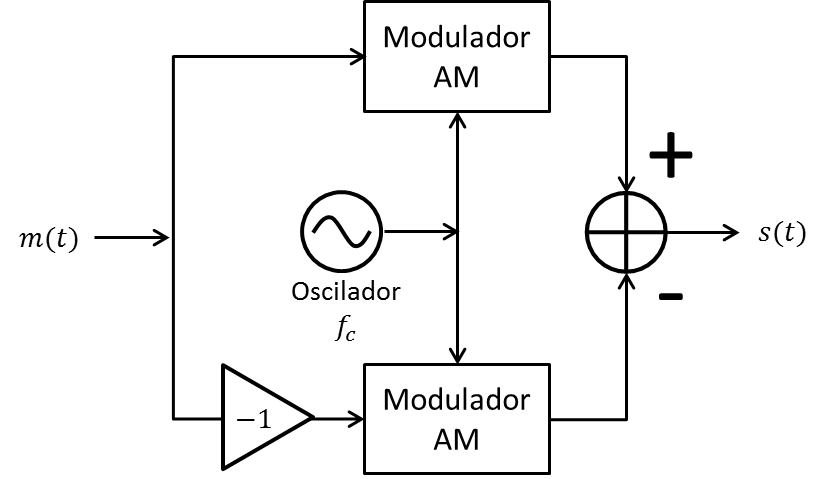
\includegraphics[scale=0.65]{Imagenes/2014ESQUEMA.png}
	\label{fig:2014ESQUEMA}
	%	\captionsetup{justification=raggedright,font={scriptsize,bf,it}}
	%	\caption*{fuente: llllll}
\end{figure}

%\begin{center}
%	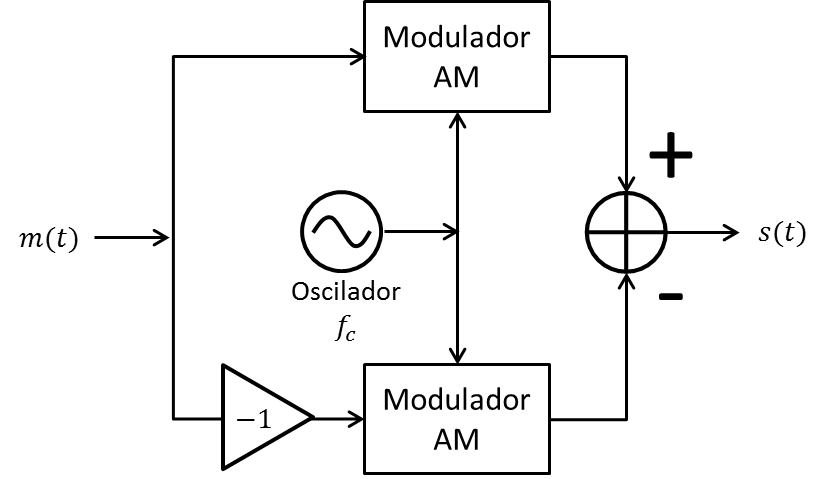
\includegraphics[scale=0.65]{imagenes/2014ESQUEMA.png} 
%\end{center}


\begin{enumerate}
	\item Usando expresiones matemáticas para describir las señales en los diferentes puntos de la figura, determine a qué clase de señal (tipo de modulación) corresponde la salida $s(t)$.
	\item Mencione una ventaja y una desventaja de este tipo de modulador.
\end{enumerate}
%%%%%%%%%%%%%%%%%%%%%%%%%%%13
\item~ Sea señal FM $s(t) = \frac{20}{10}\cos(2\pi f_c t+2\pi k_f \int{m(\tau)d\tau})$, donde la señal modulante es $m(t)=A_m \sin(2\pi f_m t + \phi)$, con $k_f=10$~kHz/V, $f_m=	10$~kHz y $A_m = 2$~V.

\begin{enumerate}
	\item~ Dibuje la densidad espectral de potencia de $s(t)$ en [dBm].
	\item~ Determine el porcentaje total de potencia de $s(t)$ que se encuentra en el rango de frecuencias.
	
	$[(f_c - 3.5f_m) , f_c + 0.5f_m]$
	
	\item~ Calcule el ancho de banda dos métodos diferentes si ahora $A_m = 10$~V.
	
	
	\item~ Responda breve y claramente qué ocurre con el espectro de $s(t)$ comparado con el literal $(a)$ si: \\
	
	\begin{itemize}
		\item Se duplica $f_m$ y se duplica $k_f$.
		\item Se duplica $f_m$ se divide en dos $A_m$.
		\item Se divide en dos $f_m$ y se amplifica $A_m$.
	\end{itemize}
	
\end{enumerate}
%%%%%%%%%%%%%%%%%%%%%%%%%%14
\item~ Se tiene un sistema de modulación como el mostrado en la siguiente figura:

\begin{figure}[h!]
	\captionsetup{justification = raggedright, singlelinecheck = false}
	\caption{Sistema de modulación} 
	\centering
	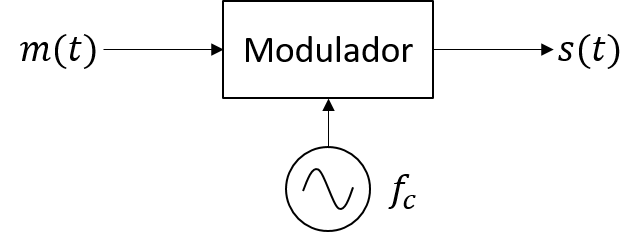
\includegraphics[scale=0.38]{Imagenes/Modulador.png}
	\label{fig:Modulador}
	%	\captionsetup{justification=raggedright,font={scriptsize,bf,it}}
	%	\caption*{fuente: llllll}
\end{figure}
%\begin{center}
%	\includegraphics[scale=0.38]{imagenes/modulador.png}
%\end{center}
donde $f_c=(600-10N)$~kHz, y la relación entrada-salida corresponde a uno de los siguientes casos:
\begin{itemize}
	\item~[CASO A:] $s(t)=3\cos(2\pi f_c t)-0,4m(t)\cos(2\pi f_c t)$~[V]
	\item~[CASO B:] $s(t)=m(t)\cos(2\pi f_c t)$~[V]
	\item~[CASO C:]  $s(t)=6\cos[2\pi f_c t+10^4\pi\int{m(\tau)d\tau}]$~[V]
	\item~[CASO D:] $s(t)=2\cos[2\pi f_c t+0,1m(t)]$~[V]
\end{itemize}
Suponiendo que la entrada del modulador es $m(t)=3+2\cos(10^4\pi t)$~[V]:
\begin{enumerate}
	\item~ Para cada relación entrada-salida del modulador, grafique la correspondiente densidad espectral de potencia de $s(t)$ (escoja escalas adecuadas para una correcta representación):

%\begin{table}[h]
%	\centering
%	\scalebox{0.80}{
%		\begin{tabular}{cll}
%			\multirow{15}{*}{
				
%				\begin{figure}[h!]
%					\captionsetup{justification = raggedright, singlelinecheck = false}
%					\caption{Sin nombre} 
%					\centering
%					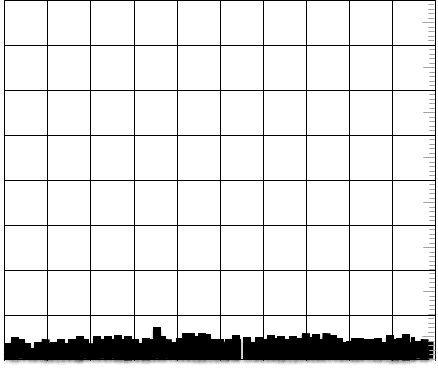
\includegraphics[scale=0.6]{Imagenes/Pantalla.png}
%					\label{fig:Pantalla}
					%	\captionsetup{justification=raggedright,font={scriptsize,bf,it}}
					%	\caption*{fuente: llllll}
%				\end{figure}								
				%	\includegraphics[scale=0.6]{imagenes/pantalla.png}
%			}
%			\\& Ref. level: &\line(1,0){60}~[dBm] \\ & & \\
%			& Central freq.:& \line(1,0){60}~[kHz] \\ & & \\
%			& dB/div: &\line(1,0){60}\\ & & \\
%			& SPAN/div: &\line(1,0){60}~[kHz]\\  & & 
%			\\
%			\\
%			\\
%			\\
%			\\
%			\\
%	\end{tabular}}
%	\caption{Alguna descripción.}
%	\label{tabla:Marco}
%\end{table}
	
	\item~ Para cada caso encuentre si es posible o no determinar:
	
	\begin{itemize}
		
		\item~ Tipo de modulación
		\item~ Índice de modulación
		\item~ Potencia de $s(t)$ [dBm]
		\item~ Ancho de banda de $s(t)$
		
	\end{itemize}
	
\end{enumerate}

%%%%%%%%%%%%%%%%%%15

\item~
Se desea usar el modulador de la siguiente figura para transmitir dos mensajes  bandabase, $m_1(t)$ y $m_2(t)$, cada una con ancho de banda $B$ y potencia $10$~mW, siendo los filtros ideales de ganancia 1, y la portadora con amplitud $A_c=5$~[V].
%\begin{center}
%	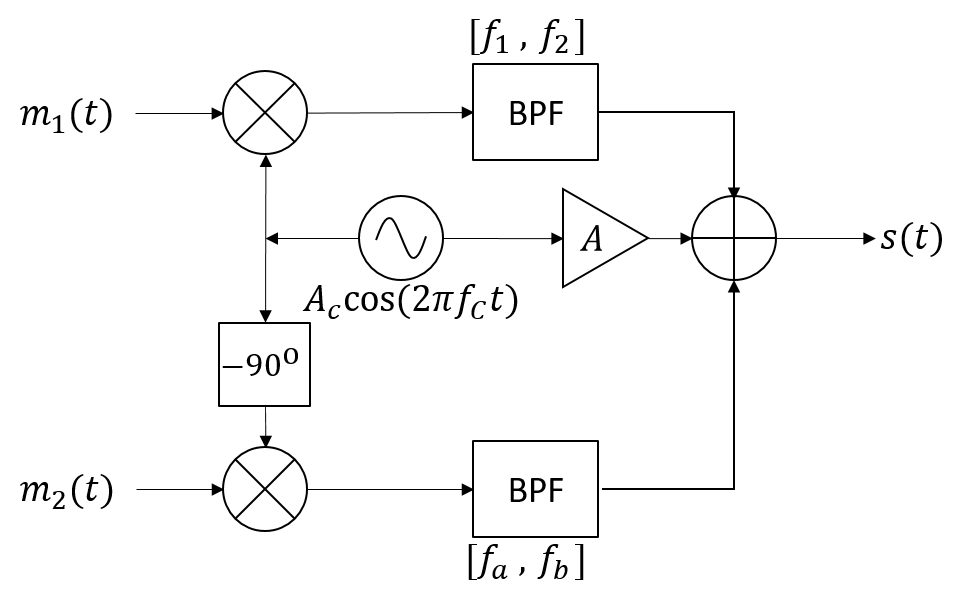
\includegraphics[scale=0.4]{imagenes/qam.png}
%\end{center}

	\vspace{200px}
\begin{figure}[h!]
	\captionsetup{justification = raggedright, singlelinecheck = false}
	\caption{Sistema de modulación} 
	\centering
	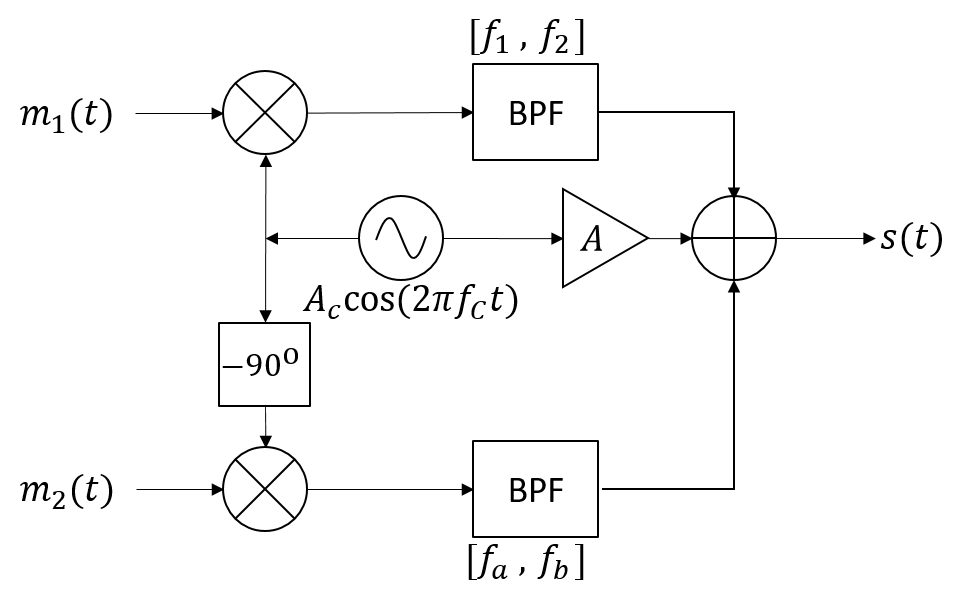
\includegraphics[scale=0.4]{Imagenes/qam.png}
	\label{fig:qam}
	%	\captionsetup{justification=raggedright,font={scriptsize,bf,it}}
	%	\caption*{fuente: llllll}
\end{figure}
Considerando las siguientes alternativas:
\begin{center}
	\begin{tabular}{cccccc}
		CASO & $A$~[V/V] & $f_1$ & $f_2$ & $f_a$ & $f_b$ \\ \hline
		I & 0 & $f_c-B$ & $f_c$ & $f_c$ & $f_c+B$ \\
		II & 1 & $f_c-B$ & $f_c+B$ & $f_c-B$ & $f_c+B$ \\
		III & 1 & $f_c$ & $f_c+B$ & $f_c$ & $f_c+B$ \\
	\end{tabular}
\end{center}
\begin{enumerate}
	\item~ ¿Cuál corresponde a una modulación QAM? Calcule la respectiva potencia (en dBm) de $s(t)$.
	
	\item~ ¿Cuál corresponde a una multiplexión por división de frecuencia? Dibuje un diagrama de bloques de un sistema que permita recuperar $m_1(t)$ y $m_2(t)$.
	
	\item~ ¿Cuál permite recuperar $m_1(t)$ sin necesidad de usar un detector coherente? Explique cómo sería posible lograr esta recuperación.
	
	\item~ ¿Cuál NO permite recuperar ninguno de los mensajes? Justifique su respuesta. 
	
\end{enumerate}
\end{enumerate}

%%%%%%%%%%%%Final modulación de onda continua

\pagebreak
\begin{center}
	\textbf{PATRÓN TRAPEZOIDAL}
	\\

\end{center}

\begin{enumerate}
	\item~ Una señal AM $s(t)$ modulada por un tono $m(t)$, tiene un patrón trapezoidal como se muestra en la siguiente figura. Tenga en cuenta que (X: 1 V/div) y (Y:4 V/div)
%	\begin{center}
%		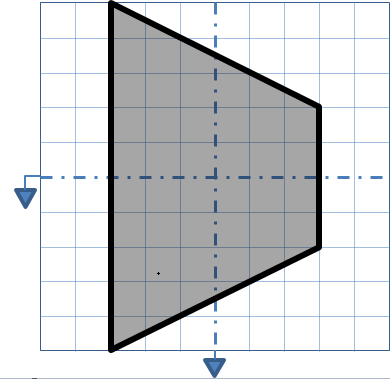
\includegraphics[scale=1]{imagenes/trap1.PNG} 
%	\end{center}	

	\begin{figure}[h!]
		\captionsetup{justification = raggedright, singlelinecheck = false}
		\caption{Patrón trapezoidal} 
		\centering
		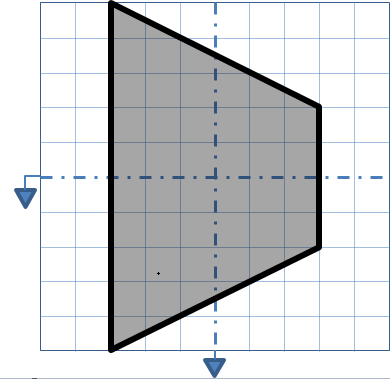
\includegraphics[scale=1]{Imagenes/trap1.png}
		\label{fig:trap1}
		%	\captionsetup{justification=raggedright,font={scriptsize,bf,it}}
		%	\caption*{fuente: llllll}
	\end{figure}

	\begin{enumerate}
		\item Calcule $k_a$ (no olvidar las unidades).
		%
		\item Calcule $\mu$.
		
		\item Calcule la potencia de $s(t)$ (en dBm).
		
		
		\item Determine una expresión para $s(t)$.
		
		\item Dibuje la densidad espectral de potencia de $s(t)$ vista en un analizador de espectros (indique las escalas apropiadas).
		\begin{center}
			Ref. level: \line(1,0){60}, Span/div: \line(1,0){60}, Center Frequency: \line(1,0){60}
			
	\begin{figure}[h!]
		\captionsetup{justification = raggedright, singlelinecheck = false}
		\caption{Densidad espectral de potencia en un analizador de espectros} 
		\centering
		
\includegraphics[scale=0.6]{Imagenes/img2.png}
		\label{fig:img2}
		%	\captionsetup{justification=raggedright,font={scriptsize,bf,it}}
		%	\caption*{fuente: llllll}
	\end{figure}	
		
		
			
		%	
\includegraphics[scale=0.6]{imagenes/img2.png} 	
		\end{center}
		\item Dibuje el patrón trapezoidal si se amplifica el mensaje en un factor de 7/3 y se le agrega un \textit{offset} de 8 [V].
		
		
	\end{enumerate}

	%%%%%%%%%%%%%%%%%%2

\item~ Una señal AM $s(t)$ con frecuencia de portadora $f_c = 980$~kHz, con potencia de portadora sin modular $P_c$, modulada por un tono de prueba, se observa en un analizador de espectros como se muestra en la siguiente figura:
\vspace{50px}
	\begin{figure}[h!]
	\captionsetup{justification = raggedright, singlelinecheck = false}
	\caption{Analizador de espectros} 
	\centering
	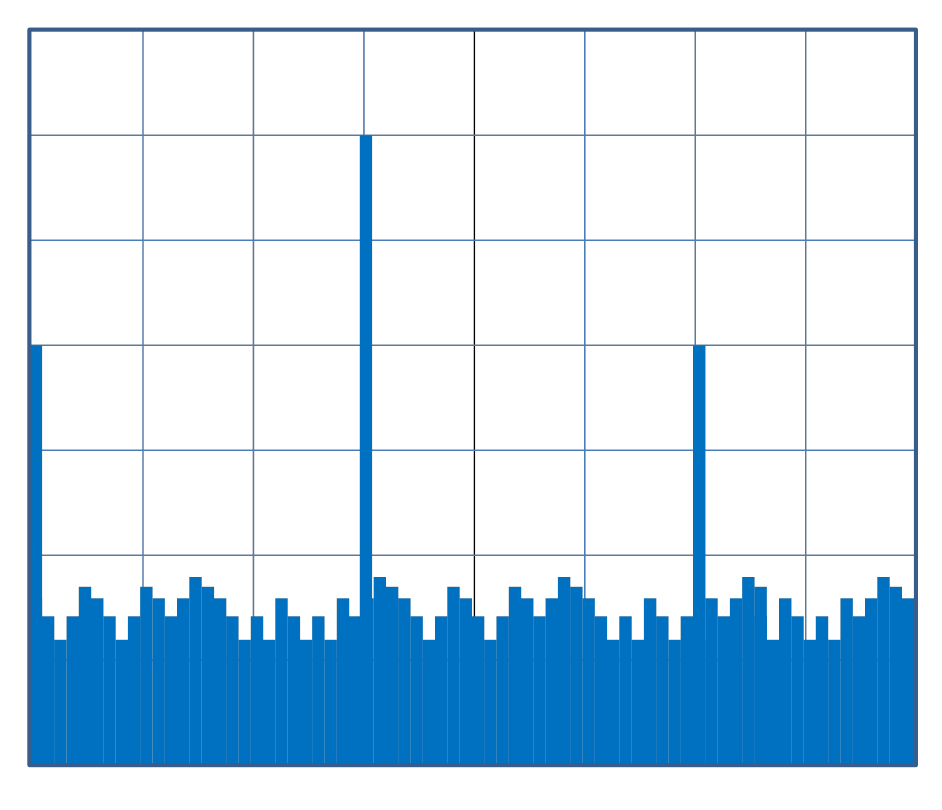
\includegraphics[scale=0.5]{Imagenes/fig4.png}
	\label{fig:fig4}
	%	\captionsetup{justification=raggedright,font={scriptsize,bf,it}}
	%	\caption*{fuente: llllll}
\end{figure}

%\begin{center}
%	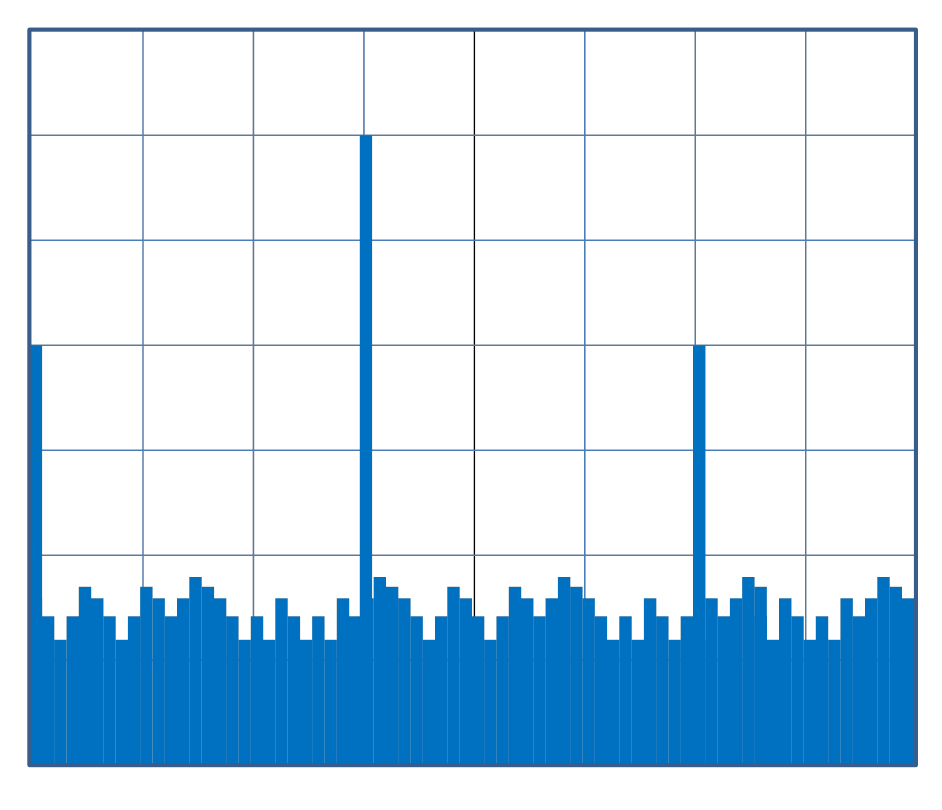
\includegraphics[scale=0.3]{imagenes/fig4.png} 
%\end{center}
donde:
\begin{itemize}
	\item Ref. Level: -10 dBm
	\item 10 dB/div
	\item CF: 990 kHz
	\item SPAN: unknown
\end{itemize}
Si se sabe que el analizador hace un barrido de frecuencias negativas y positivas, determine:

\begin{enumerate}
	\item Índice de modulación.
	
	\item Potencia total en dBm
	
	\item Eficiencia de potencia.
	
	\item La señal modulada $s(t)$.
	
	\item Patron trapezoidal.
	
	\item SNR [dB] de la portadora.
	
\end{enumerate}
%%%%%%%%%%%%%%%%%%%3
\item~ De una señal AM $s(t)$ modulada por un tono $m(t)$ de frecuencia 10~kHz se obtiene en un osciloscopio el siguiente patrón trapezoidal. Tenga en cuenta que (X:1 V/div) y (Y:4 V/div). 


	\begin{figure}[h!]
	\captionsetup{justification = raggedright, singlelinecheck = false}
	\caption{Patrón trapezoidal} 
	\centering
	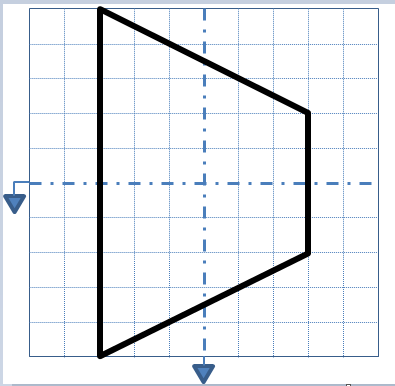
\includegraphics[scale=0.9]{Imagenes/trap2.png}
	\label{fig:trap2}
	%	\captionsetup{justification=raggedright,font={scriptsize,bf,it}}
	%	\caption*{fuente: llllll}
\end{figure}


%\begin{center}
%	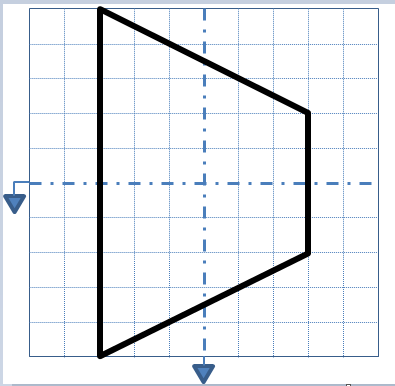
\includegraphics[scale=0.7]{imagenes/trap2.PNG} 
%\end{center}


Con base en esta información:
\begin{enumerate}
	\item~ Mencione dos (2) características de la señal modulada que se pueden identificar directamente (sin realizar ningún cálculo) de este patrón trapezoidal . Explique brevemente.
	
	\item~ Dibuje la densidad espectral de potencia de $s(t)$ vista en un analizador de espectros (indique las escalas apropiadas).
	\begin{center}
		Ref. level: \line(1,0){60}, Span/div: \line(1,0){60}, 
		
		Center Frequency: \line(1,0){60}, dB/div: \line(1,0){60}, 


	\begin{figure}[h!]
		\captionsetup{justification = raggedright, singlelinecheck = false}
		\caption{Analizador de espectros} 
		\centering
		
\includegraphics[scale=0.6]{Imagenes/img002.png}
		\label{fig:iimg002}
		%	\captionsetup{justification=raggedright,font={scriptsize,bf,it}}
		%	\caption*{fuente: llllll}
	\end{figure}	
	%	
\includegraphics[scale=0.6]{imagenes/img002.png} 
	\end{center}	
	
	
	\item La amplitud de la portadora.
	\item El índice de modulación.
	\item El coeficiente de sensibilidad del modulador.
	
\end{enumerate}

%%%%%%4
\item~ Considere una señal AM $s(t)= 20 [1+k_a m(t)]\cos((1) \times 10^6 \pi t)$~[V], con impedancia de transmisión de 50~$\Omega$, potencia total 37~dBm, modulada por $m(t)=  \cos(2000\pi t)+\sin(2000\pi t)$~[V].
\begin{enumerate}
	\item Calcule la potencia de portadora$P_c$ en [dBm]. 
	\item Calcule la potencia  $P_B [dBm] $ de las bandas laterales en [dBm]. 
	\item Obtenga $k_a$.
	\item Grafique $s(t)$ vs $m(t)$. Indique claramente la escala.
	
	\item Dibuje el espectro de potencia de $s(t)$ en la pantalla de analizador de espectros de la siguiente figura:
	
    \vspace{300px}	
	\begin{figure}[h!]
	\captionsetup{justification = raggedright, singlelinecheck = false}
	\caption{Analizador de espectros} 
	\centering
	
\includegraphics[scale=0.7]{Imagenes/img002.png}
	\label{fig:iiimg003}
	%	\captionsetup{justification=raggedright,font={scriptsize,bf,it}}
	%	\caption*{fuente: llllll}
\end{figure}

	Escogiendo adecuadamente los parámetros de configuración para una correcta visualización:
	\begin{itemize}
		\vspace{1mm}
		\item Nivel de referencia: 
		\item Escala vertical: 
		\item Frecuencia central: 
		\item Escala horizontal: 
	\end{itemize}
	\item Determine el valor de $k_a$ necesario para que el porcentaje de modulación negativo sea 100\%. 
\end{enumerate}

%%%%%%%%%%%5
\item~ Observe los siguientes patrones obtenidos al graficar una señal modulada $s(t)$ contra su respectiva señal modulante $m(t)$ (la escala es: $X: 1$~V/div; $Y: 4$ V/div). 


\begin{figure}[h!]
	\captionsetup{justification = raggedright, singlelinecheck = false}
	\caption{Patrones trapezoidales} 
	\centering
	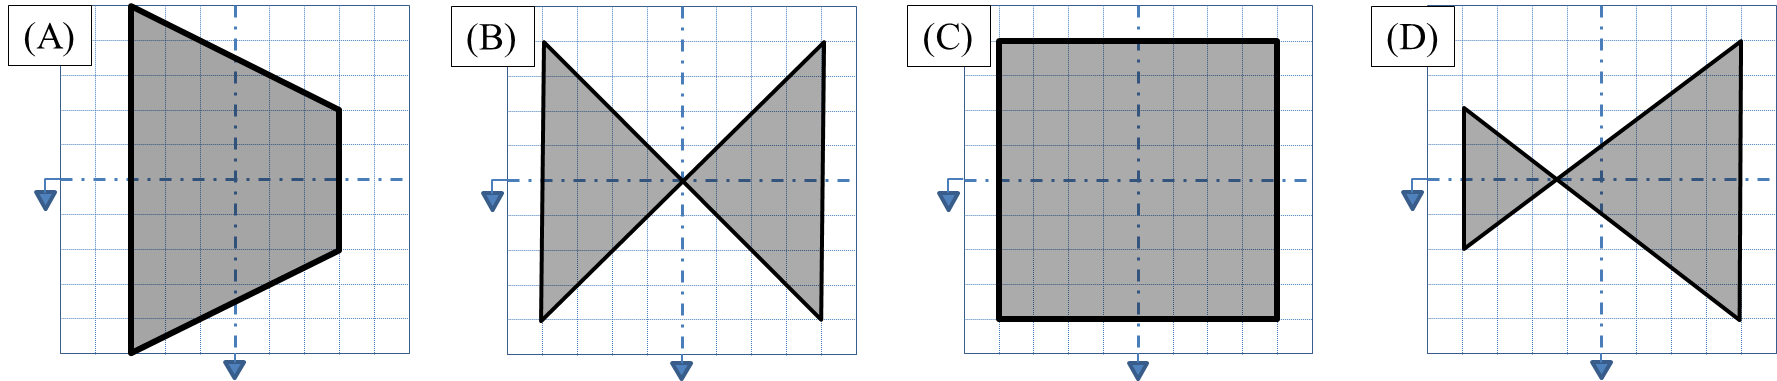
\includegraphics[scale=0.55]{Imagenes/fig05.png}
	\label{fig:fig05}
	%	\captionsetup{justification=raggedright,font={scriptsize,bf,it}}
	%	\caption*{fuente: llllll}
\end{figure}
%\begin{center}
%	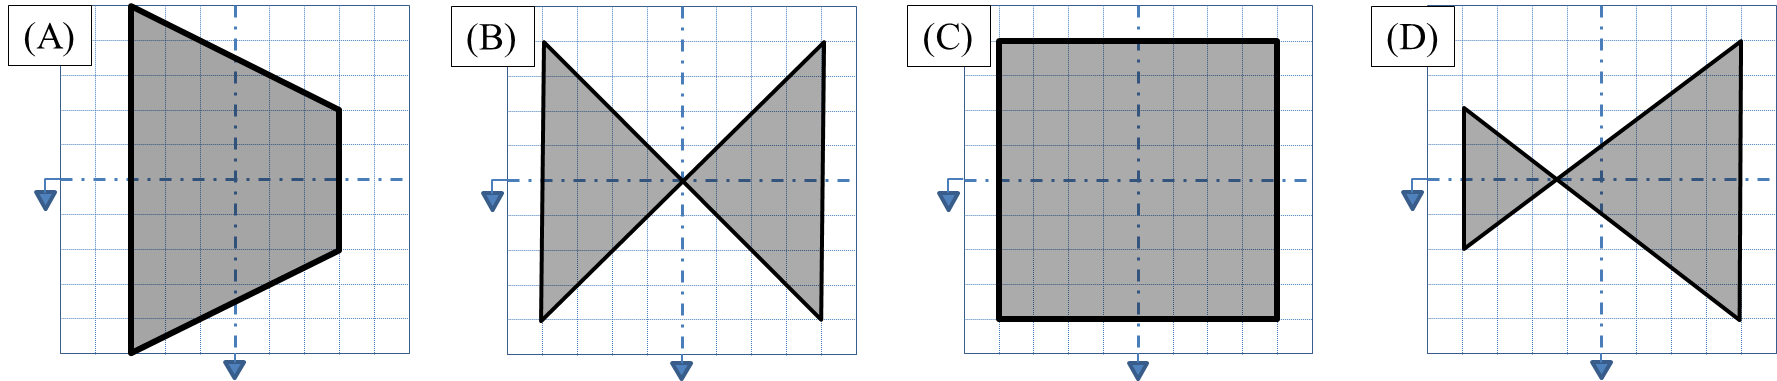
\includegraphics[scale=0.55]{imagenes/fig05.png} 
%\end{center}
Si se sabe que en todos los casos la señal modulante $m(t)$ es un tono puro:
\begin{enumerate}
	\item Identifique un tipo de modulación que corresponda a cada patrón.
	\item Encuentre una expresión matemática para cada tipo de modulación. Encuentre las constantes respectivas donde sea posible.
	\item Calcule el índice de modulación donde sea posible.
	\item Escoja un patrón correspondiente a una señal AM y elija uno de los siguientes parámetros: amplitud de portadora ($A_c$), amplitud del mensaje ($A_m$) o coeficiente de sensibilidad ($k_a$). Dibuje el patrón trapezoidal que se obtiene al modificar el parámetro escogido de tal forma que el índice de modulación sea 1.
\end{enumerate}
%%%%%%%%%%%%%%%%%%%%6
	
\item~ Una señal AM $s(t) = A \cos(2\pi f_c t) + B m(t)\cos(2\pi f_c t)$~[V], con $m(t)=C \left[ \cos(2\pi f_m t)+\cos(4\pi f_m t) \right]$, $f_m=10$~[kHz] presenta el siguiente patrón trapezoidal:


\begin{figure}[h!]
	\captionsetup{justification = raggedright, singlelinecheck = false}
	\caption{Señal AM} 
	\centering
	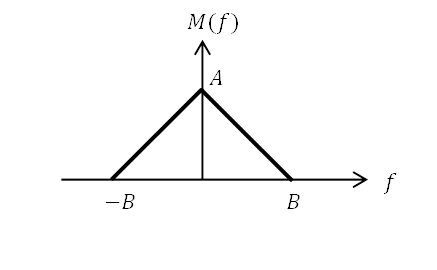
\includegraphics[scale=1]{Imagenes/fig3a.png}
	\label{fig:fig3a}
	%	\captionsetup{justification=raggedright,font={scriptsize,bf,it}}
	%	\caption*{fuente: llllll}
\end{figure}

%\begin{center}
%	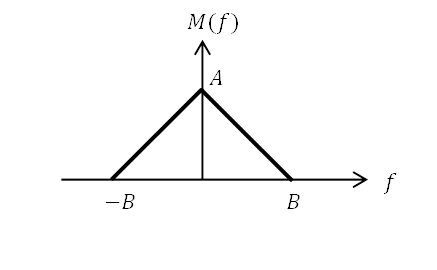
\includegraphics[scale=1]{imagenes/fig3a.png}  
%\end{center}


\begin{enumerate}
	\item~ Complete la siguiente tabla:
	
	
	\begin{figure}[h!]
		\captionsetup{justification = raggedright, singlelinecheck = false}
		\caption{Tabla de ejercicios} 
		\centering
		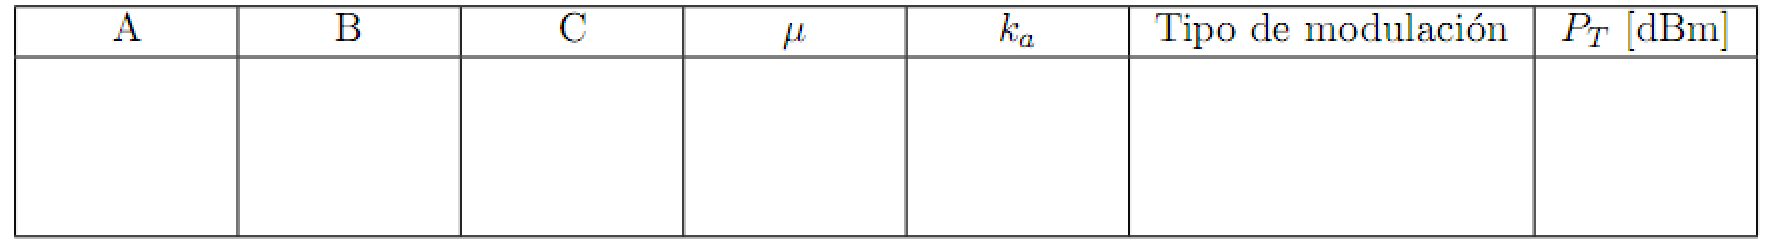
\includegraphics[scale=0.7]{Imagenes/tabla.png}
		\label{fig:tabla}
		%	\captionsetup{justification=raggedright,font={scriptsize,bf,it}}
		%	\caption*{fuente: llllll}
	\end{figure}
	
%	\begin{center}
%		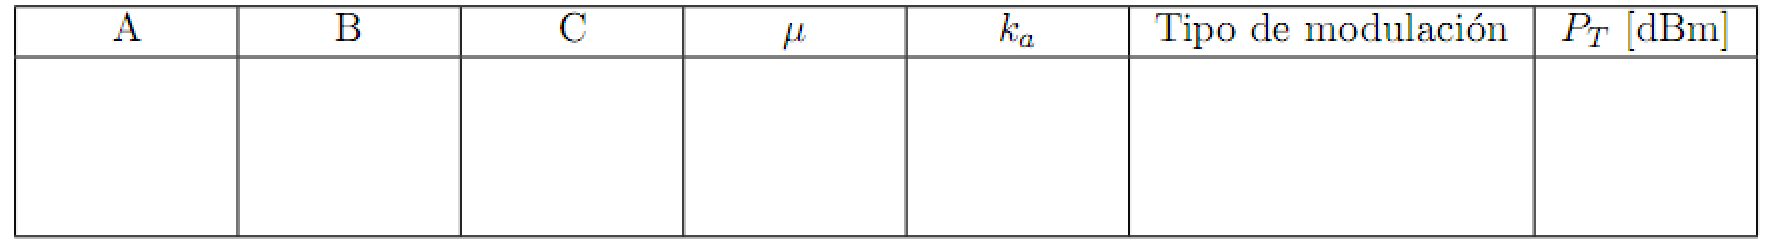
\includegraphics[scale=0.7]{imagenes/tabla.PNG} 
%	\end{center}
	
	
	\item~ Dibuje el diagrama de bloques de un demodulador para recuperar la señal $m(t)$ a partir de $s(t)$.
\end{enumerate}	
\end{enumerate}


%%%%%%%%%%%%%%%%%%%%%%%%%%%%%%%%%%%%%%%%% TALLER 3 %%%%%%%%%%%

\pagebreak
\begin{enumerate}
	\item \textbf{PREGUNTAS TEÓRICAS}
	\\
	
	
	\begin{enumerate}
		\item Responda breve y claramente:
		\begin{enumerate}
			\item Defina código de línea, de fuente y de canal  y de un ejemplo.
			\item Enuncie una ventaja y una desventaja de las modulaciones digitales comparadas con las analógicas.
			\item Enuncie una ventaja de cada una de las siguientes modulaciones de pulsos: PAM,PWM,PPM.
			\item Defina diagrama de constelación.
			
			\item Defina interferencia entre símbolos Y patrón de ojo.
			
		\end{enumerate}
		\item Obtenga los diferentes enunciados verdaderos posibles, escogiendo UNA (1) palabra de cada uno de los grupos que se encuentran entre paréntesis.
		
		\begin{enumerate}
			\item El teorema de codificación de \textbf{(fuente/canal)} establece un límite fundamental al cual la información de la fuente puede ser \textbf{(comprimida/transmitida)} sin \textbf{(pérdidas/errores)}.
			
			\item 
			En un sistema \textbf{(PCM/DPCM)} el valor de una muestra \textbf{(sí/no)} tiene efecto en la cuantización de la muestra siguiente.
			
			\item 
			La codificación de \textbf{(línea/fuente/canal)} permite transmitir \textbf{(menor/la misma/mayor)} cantidad de información en un \textbf{(menor/mismo/mayor)} ancho de banda.
			
			\item  
			El \textbf{(patrón de ojo/filtro acoplado/filtro coseno alzado)} se utiliza en la \textbf{(transmisión/recepción)} de señales digitales con el fin de \textbf{(evaluar/mitigar)} los efectos de \textbf{(ruido en el canal / interferencia entre símbolos)}
			
			\item  
			El multiacceso por división de \textbf{(frecuencia/tiempo/espacio)} requiere un estricto control de \textbf{(sincronización/potencia/ancho de banda)} de las señales que comparten el medio. 
			
			\item  
			Una \textbf{(ventaja/desventaja)} de \textbf{(PAM/PWM/PCM)} sobre \textbf{(PAM/PWM/PCM)} es su eficiencia \textbf{(espectral/de potencia/frente al ruido)}.
			\item En términos prácticos, una señal \textbf{(SÍ/NO)} puede ser reconstruida de forma \textbf{(APROXIMADA/EXACTA)} a partir de muestras cuantizadas pues, entre otras, 
			\begin{enumerate}
				\item[a)]	se requiere un filtro no realizable que  atenúe completamente un rango de frecuencias.
				\item[b)]	las señales reales son limitadas en tiempo y por tanto no son exactamente limitadas en frecuencia.
				\item[c)]	la cuantización siempre introduce error.
				\item[d)]	no es posible generar un tren de impulsos ideales.
			\end{enumerate}
			
			\item La modulación PCM es \textbf{(EFICIENTE/INEFICIENTE)} en términos de ancho de banda ya que 
			\begin{enumerate}
				\item[a)]	la tasa de muestreo debe exceder la tasa de Nyquist asociada a la señal mensaje.
				\item[b)]	en el proceso de cuantización la relación señal a ruido varía con la potencia de la señal.
				\item[c)]	las ondas cuadradas tienen potencia considerable en armónicos de alta frecuencia.
				\item[d)]	el número de niveles de cuantización usados debe ser potencia de 2.
			\end{enumerate}
			
			\item Tres criterios importantes para comparar códigos de \textbf{(FUENTE/LÍNEA/CANAL)} son:
			\begin{enumerate}
				\item[a)]	Bits por símbolo, eficiencia de potencia y ancho de banda.
				\item[b)]	Eficiencia de potencia, ancho de banda  y distribución espectral.
				\item[c)]	Ancho de banda, forma de onda y relación señal a ruido.
				\item[d)]	Interferencia intersímbolos, eficiencia de potencia y ancho de banda.
			\end{enumerate}
			
			\item La \textbf{(ENTROPÍA/CODIFICACIÓN)} de \textbf{(CANAL/FUENTE)} puede definirse como
			\begin{enumerate}
				\item[a)]	la asignación de la longitud de palabras basada en cantidad de información en un mensaje.
				\item[b)]	la adición de bits de redundancia a un mensaje digital como medio de detección o corrección de errores.
				\item[c)]	el establecimiento de la forma de onda para evitar componentes DC en la densidad espectral de potencia.
				\item[d)]	la medida de incertidumbre que describe el límite superior de la tasa de compresión para obtener una descompresión sin pérdidas.
			\end{enumerate}
			
			\item De acuerdo a la teoría de Nyquist para la transmisión sin \textbf{(ERRORES/DISTORSIÓN)}, se puede afirmar que
			\begin{enumerate}
				\item[a)]	la interferencia intersímbolos puede evitarse usando filtros convencionales.
				\item[b)]	los filtros coseno alzado se pueden implementar sin retardos.
				\item[c)]	se pueden implementar filtros básicos para reducir la interferencia intersímbolos.
				\item[d)]	es conveniente usar un filtro ideal pasabajas debido a su inmunidad frente al ruido. 
			\end{enumerate}
			\item La codificación de (línea/fuente/canal) permite la (detección de errores/compresión sin pérdidas).
			\item La modulación (PAM/PWM/PPM) no es aconsejable si se desea realizar (FDM/TDM).
			\item Las modulaciones (analógicas/digitales/pasabanda
			/bandabase) requieren en general (menor/mayor) ancho de banda que las modulaciones (analógicas/digitales
			/pasabanda/bandabase).
			\item El multiacceso por división de (frecuencia/tiempo/espacio) se emplea en sistemas de (radio AM/radio FM/telefonía móvil/televisión por cable).
			\item Una (ventaja/desventaja) de (PCM/DM) sobre (PCM/DM) se evidencia cuando (sí/no) se conoce el (rango de variación/ancho de banda) de la señal mensaje.
		\end{enumerate}
		
		\item~ Seleccione UNA (1) palabra de cada uno de los grupos que se encuentran entre paréntesis para formar un enunciado verdadero.
		\begin{enumerate}
			\item~ En un cuantizador \textbf{(lineal~/~logarítmico)}, el error de cuantización se \textbf{(mantiene~/~reduce)} \textbf{(independientemente de la~/~a menor~/~a mayor)} amplitud de la señal de entrada.
			
			\item~ El modelo OSI es útil pues con la existencia de \textbf{(determinadas~/~muchas)} tecnologías y fabricantes en el ámbito de las comunicaciones de datos, permite definir métodos \textbf{(estándar~/~específicos)} para que sistemas basados en tecnologías o de fabricantes \textbf{(similares~/~diferentes~/~rivales)} puedan comunicarse de algún modo. 
			
			\item~ En comparación con el muestreo \textbf{(natural~/~de cresta plana)}, el muestreo \textbf{(natural~/~de cresta plana)} \textbf{(no~/~sí)} genera \textbf{(ensanchamiento~/~distorsión~/~ruido)} espectral.
			
			\item~ \textbf{(Si~/~No)} es posible mantener controladas las variaciones de \textbf{(potencia~/~ancho de banda)} de una señal \textbf{(PAM~/~PWM~/~PPM)} sin importar \textbf{(la potencia~/~el ancho de banda)} del mensaje.
			
			\item~ En la modulación \textbf{(DM~/~PCM)}, \textbf{(algunas veces~/~siempre)} es necesario sobremuestrear con el fin de \textbf{(evitar~/~facilitar)} la etapa de filtrado en la \textbf{(modulación~/~demodulación)} de la señal. 
			
			\item~ Los códigos \textbf{(de línea~/~fuente~/~canal)} \textbf{(sin pérdidas~/~diferenciales~/~sin prefijos)} son robustos frente a \textbf{(ruido aditivo~/~errores de transmisión~/~errores de detección)}.
			
			\item~ Una fuente que produce los símbolos $\left\lbrace A, B, C, D \right\rbrace$ con probabilidades $\left\lbrace \right.$0.5, 0.25, 0.125, 0.125$\left. \right\rbrace$, respectivamente, tiene entropía igual a \textbf{(1~/~1.5~/~1.75~/~2)} y se puede codificar como 
			\textbf{([00, 01, 11, 10]~/~[00, 01, 10, 11]~/~[0, 10, 111, 110]~/~[0, 01, 010, 011])} para alcanzar dicho valor.
			
			\item~ El filtro \textbf{(acoplado~/~de Nyquist~/~coseno alzado)} permite \textbf{(reducir~/~mejorar~/~obtener)} la \textbf{(interferencia entre símbolos~/~relación señal a ruido~/~correlación)} entre la señal \textbf{(transmitida~/~recibida)} y la forma de los pulsos de la señal \textbf{(transmitida~/~recibida)}.
			
			\item~ La curva de tasa de error de bits (BER), medida en \textbf{(errores por segundo~/~bits por segundo)} permite valorar el desempeño de un sistema de \textbf{(transmisión~/~recepción)} en presencia de \textbf{(señal~/~ruido~/~distorsión)}.
			
			\item~ En la siguiente figura se observan las gráficas de tasa de error de bits (probabilidad de error vs relación señal a ruido en dB) para diferentes variantes de cierto código convolucional:
		
		
		
%			\begin{center}
%				\includegraphics[scale=1.0]{imagenes/ber.png}
%			\end{center}
\begin{figure}[h!]
	\captionsetup{justification = raggedright, singlelinecheck = false}
	\caption{Formación de la señal BPSK} 
	\centering
	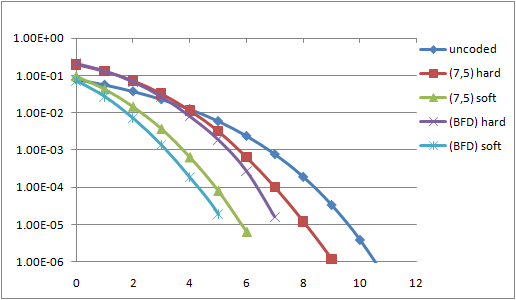
\includegraphics[scale=1]{Imagenes/Ber1.png}
	\label{fig:Ber1}
	%	\captionsetup{justification=raggedright,font={scriptsize,bf,it}}
	%	\caption*{fuente: \textcolor{
	%			Orange}{Tomada de Wikipedia}}
\end{figure}		
		
			Se observa que el uso de \textbf{([7,5]hard~/~[7,5]soft~/~[BFD]hard~/~[BFD]soft)}  \textbf{(mejora~/~empeora)} respecto a la transmisión de los datos sin codificar (\textit{encoded}) cuando la relación señal a ruido está por \textbf{(encima~/~debajo)} de los 4~dB. 
		\end{enumerate}
		
		
		
	\end{enumerate}


\newpage


\begin{center}
	\textbf{MODULACIONES DE PULSOS}
	\\
	
\end{center}


\begin{enumerate}
	%%%%%%%%%%%%%%%%%%%%%%%%%%%%%1
	\item Indique y explique brevemente una ventaja de cada uno de los códigos de línea mostrados en la siguiente figura: 

%	\begin{center}
%		\includegraphics[scale=0.4]{imagenes/linecode.png} 
%	\end{center}

\begin{figure}[h!]
	\captionsetup{justification = raggedright, singlelinecheck = false}
	\caption{Códigos de línea} 
	\centering
	\includegraphics[scale=0.4]{Imagenes/linecode.png}
	\label{fig:linecode}
	%	\captionsetup{justification=raggedright,font={scriptsize,bf,it}}
	%	\caption*{fuente: \textcolor{
	%			Orange}{Tomada de Wikipedia}}
\end{figure}
	\begin{enumerate}
		\item NRZ,AMI,CMI
		
		\item En qué capa del modelo OSI se especifica la codificación de línea de un sistema? 
	\end{enumerate}
	
	%%%%%%%%%%%%%%%%%%%%%%%%%%%%2
	\item~La señal ECG que se observa en la siguiente figura:
%	\begin{center}
%		\includegraphics[scale=0.7]{imagenes/senal-ecg.png} 
%	\end{center}

\begin{figure}[h!]
	\captionsetup{justification = raggedright, singlelinecheck = false}
	\caption{Señal ECG} 
	\centering
	\includegraphics[scale=0.7]{Imagenes/senal-ecg.png}
	\label{fig:senal-ecg}
	%	\captionsetup{justification=raggedright,font={scriptsize,bf,it}}
	%	\caption*{fuente: \textcolor{
	%			Orange}{Tomada de Wikipedia}}
\end{figure}


	Se ha muestreado a una tasa de 400~Muestras/s y se codifica PCM empleando uno de los siguientes cuantizadores cuyas funciones de respuesta normalizada son:
%	\begin{center}
%		\includegraphics[scale=0.4]{imagenes/cuantizador.png} 
%	\end{center}
\vspace{200px}
\begin{figure}[h!]
	\captionsetup{justification = raggedright, singlelinecheck = false}
	\caption{Funciones de respuesta normalizada} 
	\centering
	\includegraphics[scale=0.4]{Imagenes/cuantizador.png}
	\label{fig:cuantizador}
	%	\captionsetup{justification=raggedright,font={scriptsize,bf,it}}
	%	\caption*{fuente: \textcolor{
	%			Orange}{Tomada de Wikipedia}}
\end{figure}



	
	\begin{enumerate}
		\item ¿Cuál de los dos cuantizadores es más apropiado para digitalizar la señal ECG? Explique brevemente por qué.
		
		\item Suponga que se usa el Cuantizador 1, asignando 4 mV al nivel 000, y 7,5 mV al nivel 111. 
		\item ¿Cuál es el paso de cuantización? 
		\item ¿Cuál es el máximo error de cuantización? 
		\item Determine la capacidad de canal y ancho de banda mí­nimo, necesarios para transimitir la señal ECG modulada PCM.
		\item ¿Cuántas señales ECG como la mostrada pueden multiplexarse en un E0 (canal digital PCM de 8 bits, para señales de voz con ancho de banda de 4 kHz)?.
		
	\end{enumerate}
	%%%%%%%%%%%%%%%%%%%3
	\item Se tiene un enlace TDM de cuatro (4) canales, cada uno con una velocidad de 250~kbps.
	Cada canal se emplea para transmitir señales de audio codificadas PCM lineal, de 12 bits y resolución (paso de cuantización) de 16~mV. Determine
	\begin{enumerate}
		\item El voltaje pico a pico de la señal analógica de adecuado para este codificador.
		
		\item El ruido de cuantización (en dB) del codificador.
		
		\item La duración de cada bit.
		
		\item El ancho de banda (BW) máximo de cada señal de audio. 
		
		\item El BW aproximado del enlace, asumiendo una codificación Manchester diferencial.
		
	\end{enumerate}
%%%%%%%%%%%%%%%%%%%%%%%%%%%%4
\item~ Una señal binaria, codificada NRZ Unipolar se transmite a una tasa de 62,5~kbps a través de un canal de ancho de banda limitado y en presencia de AWGN. Algunas secuencias de bits recibidas se muestran en la siguiente figura:


%\begin{center}
%	\includegraphics[scale=0.4]{imagenes/eyepattern1.png} 
%\end{center}
\vspace{200px}
\begin{figure}[h!]
	\captionsetup{justification = raggedright, singlelinecheck = false}
	\caption{Secuencias de bits} 
	\centering
	\includegraphics[scale=0.4]{Imagenes/eyepattern1.png}
	\label{fig:eyepattern1}
	%	\captionsetup{justification=raggedright,font={scriptsize,bf,it}}
	%	\caption*{fuente: \textcolor{
	%			Orange}{Tomada de Wikipedia}}
\end{figure}



\begin{enumerate}
	\item Estime el ancho de banda del canal. Explique su criterio de estimación.
	
	\item Estime la relación señal a ruido (en dB). Explique su criterio de estimación.
	
	\item Determine aproximadamente la probabilidad de error asociada a la señal recibida.
	
	\item  Superponga las ocho (8) gráficas de la figura. Esboce y describa el resultado. 



%	\begin{center}
%		\includegraphics[scale=0.55]{imagenes/template1.png} 
%	\end{center}

\begin{figure}[h!]
	\captionsetup{justification = raggedright, singlelinecheck = false}
	\caption{Tabka para describir el resultado} 
	\centering
	\includegraphics[scale=0.7]{Imagenes/template1.png}
	\label{fig:template1}
	%	\captionsetup{justification=raggedright,font={scriptsize,bf,it}}
	%	\caption*{fuente: \textcolor{
	%			Orange}{Tomada de Wikipedia}}
\end{figure}



	
	\item Observe la gráfica de la secuencia $[1 0 1]$. Comente una consecuencia de reducir el tiempo de bit a la mitad.
	
\end{enumerate}
%%%%%%%%%%%%%%%%%%%%%%%5
\item Dibuje el diagrama de bloques de un modulador PWM, asumiendo una entrada de ancho de banda  4~kHz y 10Vpp y especifique condiciones para que el ciclo útil de la señal de salida varíe exactamente entre el $10\%$ y el $90\%$. 
%%%%%%%%%%%%%%%%%%%%%%%%%%6

\item Se tiene un codificador PCM lineal, de signo y magnitud, de 12 bits y resolución de 0,016~V, cuya salida se comprime digitalmente a 8 bits. Determine
\begin{enumerate}
	\item El rango de la señal analógica de adecuado para este codificador.
	\item El ruido de cuantización (en dB) del codificador de 12 bits, y de la salida comprimida de 8 bits
	\item El código PCM de 12 bits y de 8 bits para los voltajes cuantizados: -6,592V, +12,992V y -3,36V.
	
	\item La resolución de la salida comprimida de 8 bits.
\end{enumerate}
%%%%%%%%%%%%%%%%%%7
\item Se tiene un codificador PCM lineal, de signo y magnitud, de 12 bits y resolución de 0,016~V, cuya salida se comprime digitalmente a 8 bits. Determine
\begin{enumerate}
	\item El rango de la señal analógica de adecuado para este codificador.
	\item El ruido de cuantización (en dB) del codificador de 12 bits, y de la salida comprimida de 8 bits.
	\item El código PCM de 12 bits y de 8 bits para los voltajes cuantizados: -6,592V, +12,992V y -3,36V.
	\item La resolución de la salida comprimida de 8 bits.
\end{enumerate}

%%%%%%%%%%%%%%%%%8

\item~
Se desea codificar PCM una señal de audio de 22050 Hz de ancho de banda, que varía entre $\pm 5$~[V]. Si se desea tener una resolución de al menos 1 [mV] empleando un cuantizador uniforme por redondeo, determine:
\begin{enumerate}
	\item Número de bits del cuantizador, $N$.
	
	\item Paso de cuantización, $\Delta$.
	
	\item Ancho de banda requerido para transmitir la señal codificada NRZ, $B_T$.
	
	\item Capacidad de canal necesaria para transmitir la señal codificada, $C$.
	
	\item ¿Cuántas señales PCM codificadas como ésta se pueden multiplexar en un canal de 2048 kbps?
	
	\item Capacidad de canal necesaria para transmitir la señal codificada, incluyendo un bit de paridad por cada muestra de la señal de audio.
\end{enumerate}

%%%%%%%%%%%%%%%%%%%%%%%%%%%%%9

\item~
En la siguiente figura, se ilustra la codificación Manchester de una señal. \\

%\begin{center}
%	\includegraphics[scale=0.7]{imagenes/codlinea.png}
%\end{center}

\begin{figure}[h!]
	\captionsetup{justification = raggedright, singlelinecheck = false}
	\caption{Codificación Manchester de una señal} 
	\centering
	\includegraphics[scale=1]{Imagenes/codlinea.png}
	\label{fig:codlinea}
	%	\captionsetup{justification=raggedright,font={scriptsize,bf,it}}
	%	\caption*{fuente: \textcolor{
	%			Orange}{Tomada de Wikipedia}}
\end{figure}

Asumiendo una tasa de transmisión de 1 Mbps:\\
\begin{enumerate}
	\item~ Asigne una escala apropiada de tiempo en la figura anterior.
	
	\vspace{2mm}
	
	\item~ ¿Cuál es el ancho de banda aproximado de la señal codificada?
	
	\vspace{2mm}
	
	\item~ Enuncie dos ventajas de esta codificación frente a la NRZ bipolar.
	
\end{enumerate}
%%%%%%%%%%%%%%%%%%%%%%%%%10


\item~ Un puerto serial está configurado para recibir 8 bits por símbolo, incluyendo un bit de paridad (par). Si el puerto recibe la siguiente señal NRZ bipolar correspondiente a un símbolo:


%\begin{center}
%	\includegraphics[scale=1.4]{imagenes/serial.png}
%\end{center}

\begin{figure}[h!]
	\captionsetup{justification = raggedright, singlelinecheck = false}
	\caption{Señal NRZ bipolar} 
	\centering
	\includegraphics[scale=1.4]{Imagenes/serial.png}
	\label{fig:serial}
	%	\captionsetup{justification=raggedright,font={scriptsize,bf,it}}
	%	\caption*{fuente: \textcolor{
	%			Orange}{Tomada de Wikipedia}}
\end{figure}

\begin{enumerate}
	\item~ ¿Cuál es la velocidad de transmisión?
	
	\item~ ¿Hay error en el dato recibido? Explique.
	
	\item~ La probabilidad de error de la señal recibida se puede estimar como $P_e=0,5\mbox{erfc}(\sqrt{E_b/N_0})$, determine:
	\begin{itemize}
		\item La probabilidad de error, $P_e$.
		
		\item La tasa de errores por segundo que recibe el puerto cuando el nivel de ruido es igual al de la señal.
		
		\item La relación señal a ruido (en dB) mínima para que la probabilidad de error sea inferior a un error por cada 8 bits transmitidos.
	\end{itemize}
\end{enumerate}
\end{enumerate}



\newpage
\begin{center}
	\textbf{TRANSMISIÓN DE PULSOS BANDABASE}
	\\
	
\end{center}

\begin{enumerate}
	\item Una trama T1 está compuesta por 193 bits/trama, que corresponden a 24 canales de voz de PCM de 7 bits, más un bit de señalización al final de cada muestra, además de un bit de conformación al inicio de cada trama, que se transmite a una tasa de 8000 tramas por segundo.
	
%	\begin{center}
%		\includegraphics[scale=0.65]{imagenes/tramat1.png} 
%	\end{center}	
\begin{figure}[h!]
	\captionsetup{justification = raggedright, singlelinecheck = false}
	\caption{Tramas T1} 
	\centering
	\includegraphics[scale=0.65]{Imagenes/tramat1.png}
	\label{fig:tramat1}
	%	\captionsetup{justification=raggedright,font={scriptsize,bf,it}}
	%	\caption*{fuente: \textcolor{
	%			Orange}{Tomada de Wikipedia}}
\end{figure}	
	Por otra parte, una trama E1 está compuesta por 256 bits/trama, que corresponden a 30 canales de voz PCM de 8 bits y dos canales de sincronización de 8 bits cada uno, a una tasa de transmisión de 8000 tramas por segundo. 
	
%	\begin{center}
%		\includegraphics[scale=0.95]{imagenes/tramae1.png} 
%	\end{center}	

\begin{figure}[h!]
	\captionsetup{justification = raggedright, singlelinecheck = false}
	\caption{Tramas E1} 
	\centering
	\includegraphics[scale=1.0]{Imagenes/tramae1.png}
	\label{fig:tramae1}
	%	\captionsetup{justification=raggedright,font={scriptsize,bf,it}}
	%	\caption*{fuente: \textcolor{
	%			Orange}{Tomada de Wikipedia}}
\end{figure}		
	Con base en lo anterior determine:
	
	\begin{enumerate}
		\item~ El ancho de banda máximo de cada señal de voz transmitida en una trama T1 y de una trama E1.
		
		\item La duración de cada bit en las tramas T1 y E1.
		\item La mínima relación señal a ruido que teóricamente se puede permitir si se desea transmitir información del T1 y E1 prácticamente libre de errores.
		
		\item La velocidad del canal digital binario para transmitir tramas T2 y E2, si se sabe que éstas se componen por 4 tramas T1 y 4 tramas E1, respectivamente. 
		
		\item Los requerimientos de ancho de banda mínimos si para esta trasmisión se emplea un filtro coseno alzado con un factor de roll-off de 1.0, con el fin de disminuir la interferencia intersímbolo en la trasmisión de una trama T2.
		
	\end{enumerate}
	%%%%%%%%%%%%%%%%%%%%%%%%%%%2
	\item Considere un canal inalámbrico donde la potencia recibida decrece en relación con la distancia de acuerdo con la expresión $P(d)$[W]$=P_T(d_0/d)^3$, siendo $P_T$[W] la potencia transmitida y $d$ la distancia del enlace. Asuma que $d_0=10$~m y la potencia transmitida es de 60~dBm, además de una densidad espectral de ruido de $10^{-14}$~W/Hz.
	
	Si se desea transmitir una señal digital binaria de 10~Mbps a través de un ancho de banda de 6~MHz del canal inalámbrico descrito, determine:
	
	\begin{enumerate}
		
		\item La máxima distancia $d_{\mbox{máx}}$ a la que se puede ubicar el receptor.
		\item Si el receptor se encuentra a 1000 m de distancia, ¿cuál debe ser la potencia mínima de la señal transmitida?
		
		\item  La probabilidad de error y tasa de error por segundo, si se emplea codificación NRZ para transmitir la señal.
		
	\end{enumerate}
	%%%%%%%%%%%%%%%%%%%%%%%%%3
\item Se tiene que una trama E1 (canal digital binario de 2,048 Mbps) correspondea la TDM de 32 E0 (canales de 64 kbps c/u). Treinta E0 corresponden a sendas señales de voz codificadas PCM en 8 bits y los dos restantes son canales digitales de señalización, tal como se muestra en la siguiente figura:


%\begin{center}
%	\includegraphics[scale=0.8]{imagenes/figtramae1.png} 
%\end{center}

\begin{figure}[h!]
	\captionsetup{justification = raggedright, singlelinecheck = false}
	\caption{Tramas} 
	\centering
	\includegraphics[scale=0.8]{Imagenes/figtramae1.png}
	\label{fig:figtramae2}
	%	\captionsetup{justification=raggedright,font={scriptsize,bf,it}}
	%	\caption*{fuente: \textcolor{
	%			Orange}{Tomada de Wikipedia}}
\end{figure}

Determine: 
\begin{enumerate}
	\item El ancho de banda máximo de cada señal de voz .
	
	\item La duración de cada bit. 
	
	\item El número de tramas E1 necesarias para transmitir la información correspondiente a un (1) minuto de cada señal de voz.
	
	\item La frecuencia de muestreo si uno de los canales PCM se reemplaza por un canal DM para transmitir la misma clase de señal de voz de un E0, sin alterar la duración de la trama E1.
	
	\item ¿Cuántos E0 se requieren para transmitir audio con calidad de CD (señal estereo, de 22,05 kHz por canal y 16 bit)? 
	
	
	\item ¿Es necesario que estos E0 correspondan a canales PCM consecutivos?
	
	
	\item ¿Cuál es la mínima relación señal a ruido que teóricamente se puede permitir si se desea transmitir la la información del E1 sin errores, por un medio con ancho de banda de 1 MHz?
	
	
\end{enumerate}

%%%%%%%%%%%%%%%%%%%%%%4
\item Se tiene un enlace TDM de cinco (5) canales, cada uno con una velocidad de 250~kbps. 
Si la unidad de multiplexación es de 3 bits (número de bits de cada canal que se transmiten en forma consecutiva), determine:
\begin{enumerate}
	\item La duración de cada trama.
	\item La duración de una ranura de tiempo de salida.
	\item La tasa de bits del enlace.
	\item La duración de cada bit.
	\item Las tramas (emplee codificación octal) si en cierto momento se transmiten los siguientes datos por cada canal: 
	
	\begin{tabular}{|c|c|}
		\hline
		Canal & Datos \\
		\hline
		1 & 000111000111 \\ \hline
		2 & 101010101010 \\ \hline
		3 & 001100110011 \\ \hline
		4 & 101011001010 \\ \hline
		5 & 111111100000 \\ \hline
	\end{tabular} 
	
\end{enumerate}
%%%%%%%%%%%%%%%%%%%%%%5
\item Se desean multiplexar, empleando TDM, las siguientes señales: (16)~canales de voz, (15)~canales de datos y un (1)~canal de sincronización.
Las características de los canales son las siguientes:
\begin{itemize}
	\item Canales de voz: ancho de banda de 16~kHz, codificados PCM con relación señal a ruido de cuantización superior a los 96~dB.
	\item Canales de datos: digitales de 8 niveles y tasa de transmisión de 8~kbauds.
	\item Canal de sincronización: digital binario de 1~kbps.
\end{itemize}

Asumiendo que la señal multiplexada se transmite en 8 niveles, determine: 
\begin{enumerate}
	\item ¿Cuál es la mínima capacidad de canal requerida (en bauds y bps)?
	
	\item Según el teorema de capacidad de canal de Shannon, ¿cuál es el mínimo ancho de banda necesario para la transmisión, asumiendo una relación señal a ruido de $N$ [dB]?
	
	\item Para el caso de una transmisiòn binaria, con una relación señal a ruido $E_b/N_0=3$~dB, ¿cuántos errores estima que se producirían en un segundo en la recepción?
\end{enumerate}
\end{enumerate}




\newpage
\begin{center}
	\textbf{TEORÍA DE LA INFORMACIÓN}
	\\
\end{center}


\begin{enumerate}
	\item El alfabeto de símbolos $x_i$ de una fuente, se codifica empleando el método de Shanno-Fano, basado en entropí­a, y se obtiene el siguiente resultado:

\begin{figure}[h!]
	\captionsetup{justification = raggedright, singlelinecheck = false}
	\caption{Resultadi usando método de Shanno-Fano} 
	\centering
	\includegraphics[scale=0.4]{Imagenes/shannonfano.png}
	\label{fig:shannonfano}
	%	\captionsetup{justification=raggedright,font={scriptsize,bf,it}}
	%	\caption*{fuente: \textcolor{
	%			Orange}{Tomada de Wikipedia}}
\end{figure}

%	\begin{center}
%		\includegraphics[scale=0.4]{imagenes/shannonfano.png} 
%	\end{center}
	
	
	\begin{enumerate}
		\item Calcule la entropía de la fuente.
		
		\item Obtenga y compare la longitud promedio de la fuente codificada empleando Shannon-Fano, con la obtenida empleando Huffman (asigne '0' a las ramas de mayor probabilidad).
		
		\item Obtenga y compare la longitud en bit de la palabra ``ALEGRÍA'' codificada empleando Shannon-Fano con el resultado de emplear codificación de longitud fija.
		
		
	\end{enumerate}
	%%%%%%%%%%%%%%%%%%%%%%%%%%%%%%%%%%%%2
	\item  Se tiene una fuente que genera dígitos decimales con las siguientes probabilidades:
	
    \begin{table}[h]
		\captionsetup{justification = raggedright,singlelinecheck = false}
		\caption{Ejercicio tres.}
        \label{tabla:tabla16}
        \centering
    \scalebox{1}{

		\begin{tabular}{|l|c|c|c|c|c|c|c|c|c|c|}
			\hline
			Símbolo & 0 & 1 & 2 & 3 & 4 & 5 & 6 & 7 & 8 & 9  \\
			\hline
			Probabilidad & {0,010} & {0,150} & {0,510} & {0,030} & 
			{0,150} & {0,050} & {0,040} & {0,020} & {0,010} & {0,030}  \\
			\hline
		\end{tabular}}
\end{table}
	
	
	\begin{enumerate}
		\item  ¿Cuál es la entropía de la fuente?
		\item Encuentre el código Huffman correspondiente a la fuente. ¿Cuál es la longitud promedio (bits/símbolo) que se logra con esta codificación? 
		\item Determine la cantidad de bits que se requieren para representar su código de estudiante empleando el código obtenido en el literal anterior. ¿Cuánto se comprimió respecto a la mejor codificación de longitud fija posible? 
	\end{enumerate}
	%%%%%%%%%%%%%%%%%%%%%%%%%%%%%%%%3
	\item La siguiente tabla muestra la probabilidad de aparición de las diferentes letras del alfabeto en el idioma español:
	
\begin{table}[h]
	\centering
	\captionsetup{justification = raggedright,singlelinecheck = false}
    \caption{Probabilidad de aparición de diferentes letras del alfabeto.}
    \label{tabla:tabla17}
	\scalebox{0.80}{	

		\begin{tabular}{|c|c|c||c|c|c||c|c|c|}
			\hline
			Letra & Prob. (\%) & Cant. Inf. & Letra & Prob. (\%) & Cant. Inf. & Letra & Prob. (\%)& Cant. Inf.   \\
			\hline
			A & 12,32 && J &  0,44 && R &  6,87 &\\
			B &  1,42 && K &  0,01 && S &  7,94 &\\
			C &  4,68 && L &  4,97 && T &  4,63 &\\
			D &  5,86 && M &  3,15 && U &  3,93 &\\
			E & 13,48 && N &  6,71 && V &  0,90 &\\
			F &  0,69 && Ñ &  0,31 && W &  0,02 &\\
			G &  1,01 && O &  8,68 && X &  0,22 &\\
			H &  0,70 && P &  2,51 && Y &  0,90 &\\
			I &  6,25 && Q &  0,88 && Z &  0,52 &\\
			\hline
		\end{tabular}}
\end{table}
	
	\begin{enumerate}
		\item Complete la tabla anterior indicando la cantidad de información en [bits] de cada una de las letras del alfabeto. 
		
		\item ¿Cuál es la entropía de la fuente? 
		
		\item ¿Cuál es la cantidad de información que contiene su primer apellido escrito con este alfabeto? 
		
		\item ¿Cuántos bits son necesarios como mínimo para codificar su primer apellido empleando un código de longitud fija?
		
		
		\item Si se logra codificar la fuente con la mínima longitud promedio por símbolo posible, ¿cuál es la tasa de compresión que se lograría respecto al resultado de literal anterior?
		
		\item Enuncie una ventaja de la codificación de longitud fija y una de la codificación Huffman.
		
		\item Codificación de longitud fija: 
		
		\item Codificación Huffman.
		
	\end{enumerate}
	%%%%%%%%%%%%%%%%%%%%%%%%4
\item En un archivo con aproximadamente $10^5$ caracteres se sabe que aparecen seis (6) caracteres diferentes con las siguientes frecuencias:
\begin{table}[h]
    \captionsetup{justification = raggedright,singlelinecheck = false}
    \caption{Ejercicio d}
    \label{tabla:tabla18}
	\centering
	\scalebox{0.80}{
	\begin{tabular}{|l|c|c|c|c|c|c|}
		\hline
		Caracter & A & B & C & D & E & F   \\
		\hline
		Frecuencia (miles)  & {\large $5$} & {\large $13$} & {\large $12$} & {\large $16$} & 
		{\large $9$} & {\large $45$}    \\
		\hline
		Cód.PCM& \qquad\qquad\quad\qquad &\qquad\qquad\qquad\quad &\qquad\qquad\quad\qquad &\qquad\qquad\qquad\quad & \quad\qquad\quad\qquad& \quad\qquad\qquad\quad\\
		& & & & & & \\
		\hline
		Cód. Huffman& \qquad\qquad\quad\qquad &\qquad\qquad\qquad\quad &\qquad\qquad\quad\qquad &\qquad\qquad\qquad\quad & \quad\qquad\quad\qquad& \quad\qquad\qquad\quad\\
		& & & & & & \\
		\hline
	\end{tabular}}
\end{table}

\begin{enumerate}
	\item ¿Cuál es la entropía de la fuente? 
	
	\item Complete la tabla anterior empleando codificación PCM y codificación Huffman para representar los símbolos.  ¿Cuál es la longitud promedio (bits/símbolo) que se obtiene con cada codificación? 
	
	\item Enuncie una ventaja de la codificación PCM y una de la codificación Huffman.
	
\end{enumerate}
%%%%%%%%%%%%%%%%%%%%%%%%%%%%%%%%%%5
\item Se tiene una fuente que genera los siguientes símbolos con sus respectivas probabilidades:

\begin{table}[h]
\captionsetup{justification = raggedright,singlelinecheck = false}
\caption{Ejercicio E}
\label{tabla:tabla19}
	\centering
	\scalebox{0.80}{
	\begin{tabular}{|l|c|c|c|c|c|c|c|c|}
		\hline
		Símbolo & A & E & I & O & U & C & R & T   \\
		\hline
		Probabilidad & {\Large 0,200} & {\Large 0,250} & {\Large 0,100} & {\Large 0,150} & 
		{\Large 0,050} & {\Large 0,070} & {\Large 0,120} & {\Large 0,060}   \\
		\hline
		Cód.Huffman& & & & & & & & \\
		& & & & & & & & \\
		\hline
	\end{tabular}}
\end{table}

\begin{enumerate}
	\item ¿Cuál es la entropía de la fuente? 
	
	\item Complete la tabla anterior encontrando el código Huffman correspondiente a la fuente. ¿Cuál es la longitud promedio (bits/símbolo) que se logra con esta codificación? 
	
	\item Utilizando el código obtenido en el literal anterior, decodifique el siguiente fragmento de señal: $0001001100100010001101000...$
	
\end{enumerate}


	\end{enumerate}
%%%%%%%%%%%%%%%%%%%%%%%%%%%%%%%%%%%%%%%%%%%%%%%
\newpage


\begin{center}
	\textbf{MODULACIONES DIGITALES (pasabanda)}
	\\
	
\end{center}



\begin{enumerate}
	%%%%%%%%%%%%%%%%%%%%%%%%%%%%%1
	\item En la siguiente figura, se observa una señal digital binaria NRZ al pasar a través de: (a) un filtro ideal, (b) un filtro no ideal, (c) un filtro no ideal y en presencia de ruido.
	
	
%	\begin{center}
%		\includegraphics[scale=0.4]{imagenes/eyepattern.png} 
%	\end{center}


\begin{figure}[h!]
	\captionsetup{justification = raggedright, singlelinecheck = false}
	\caption{Señal digital binaria NRZ} 
	\centering
	\includegraphics[scale=0.3]{Imagenes/eyepattern.png}
	\label{fig:eyepattern}
	%	\captionsetup{justification=raggedright,font={scriptsize,bf,it}}
	%	\caption*{fuente: \textcolor{
	%			Orange}{Tomada de Wikipedia}}
\end{figure}	


	\begin{enumerate}
		\item Dibuje el patrón de ojo correspondiente a cada una de las variantes de la señal.
		\item Resalte (\textit{encerrando en un cí­rculo o indicando con flechas}) en cada uno de los patrones del literal $a)$, una característica identificable propia de dicho patrón, y enúncienla brevemente:
		\begin{itemize}
			\item Figura (a): Filtrado ideal
			\item Figura (b): Filtrado con ISI
			\item Figura (c): Ruido más ISI
		\end{itemize}
		\item Dibuje el patrón de ojo aproximado si la señal de la figura (a) se pasa por un segundo filtro basabajas ideal de la mitad del ancho de banda del primero.
		\item Suponiendo que $T_b=1\mu s$, estime la tasa de error de bit [errores/s] sólo por efecto de ruido aditivo, tal que $SNR = 12$~dB.
	\end{enumerate}
	%%%%%%%%%%%%%%%%%%%%%%%%%%%2
	\item Se requiere evaluar un conjunto de técnicas de modulación digital caracterizadas ante el ruido según se muestra en la siguiente figura:


%	\begin{center}
%		\includegraphics[scale=0.5]{imagenes/figcurvas.png} 
%	\end{center}
\vspace{400px}
\begin{figure}[h!]
	\captionsetup{justification = raggedright, singlelinecheck = false}
	\caption{Modulación digital caracterizadas ante el ruido } 
	\centering
	\includegraphics[scale=0.4]{Imagenes/figcurvas.png}
	\label{fig:figcurvas}
	%	\captionsetup{justification=raggedright,font={scriptsize,bf,it}}
	%	\caption*{fuente: \textcolor{
	%			Orange}{Tomada de Wikipedia}}
\end{figure}


	Si se desea enviar información a una tasa de 1 Mbps: 
	\begin{enumerate}
		\item Para cada tipo de modulación estime la cantidad de bits perdidos en el transcurso de un día cuando la relación señal a ruido es 14 dB.
		
		\item Para cada tipo de modulación estime la relación señal a ruido cuando se tiene una BER de 1 error/s. MSK, QAM,PSK,DPSK
		
		
		\item ¿Qué ventaja supone tendrá la modulación MSK respecto a las otras, considerando que es la que peor desempeño tiene ante el ruido?
		
		\item ¿En qué caso preferiría usar el sistema QAM en lugar del sistema PSK?
		
		\item Determine aproximadamente la probabilidad de error asociada a la señal recibida.
		
		
	\end{enumerate}

%%%%%%%%%%%%%%%%%%%%%%%%%%%%%%%%%%3
\item Se tiene un modulador 16QAM como se muestra en la figura:

%\begin{center}
%	\includegraphics[scale=0.65]{imagenes/16qam.jpg} 
%\end{center}


%\vspace{200px}
\begin{figure}[h!]
	\captionsetup{justification = raggedright, singlelinecheck = false}
	\caption{Modulador 16QAM } 
	\centering
	\includegraphics[scale=0.50]{Imagenes/16qam.jpg}
	\label{fig:16qam}
	%	\captionsetup{justification=raggedright,font={scriptsize,bf,it}}
	%	\caption*{fuente: \textcolor{
	%			Orange}{Tomada de Wikipedia}}
\end{figure}


Si la portadora de referencia es $-2\cos(2\pi\times 10^8 t)$:


\begin{enumerate}
	\item Determine las fases y las amplitudes de cada punto (cuadrabit) de la constelación resultante. Complete la siguiente tabla y construya la constelación. 
   % \vspace{500px}
\begin{table}[h]
\captionsetup{justification = raggedright,singlelinecheck = false}
\caption{Alguna descripción.}
\label{tabla:tabla20}
	\centering
	\scalebox{0.80}{	
	\begin{tabular}{|c|c|c|c|c|c|}
		\hline
		$Q$ & $Q'$ & $I$ & $I'$ & Fase \qquad & Amplitud \\
		\hline
		0 & 0 & 0 & 0 & & \\
		\hline
		0 & 0 & 0 & 1 & & \\
		\hline
		0 & 0 & 1 & 0 & & \\
		\hline
		0 & 0 & 1 & 1 & & \\
		\hline
		0 & 1 & 0 & 0 & & \\
		\hline
		0 & 1 & 0 & 1 & & \\
		\hline
		0 & 1 & 1 & 0 & & \\
		\hline
		0 & 1 & 1 & 1 & & \\
		\hline
		1 & 0 & 0 & 0 & & \\
		\hline
		1 & 0 & 0 & 1 & & \\
		\hline
		1 & 0 & 1 & 0 & & \\
		\hline
		1 & 0 & 1 & 1 & & \\
		\hline
		1 & 1 & 0 & 0 & & \\
		\hline
		1 & 1 & 0 & 1 & & \\
		\hline
		1 & 1 & 1 & 0 & & \\
		\hline
		1 & 1 & 1 & 1 & & \\
		\hline
	\end{tabular}}
\end{table}
	
	\item Calcule el ancho de banda y las frecuencias laterales superior e inferior sabiendo que la velocidad de la señal binaria de entrada es $f_b=10$~Mbps.
	\item Dibuje el diagrama de constelación correspondiente (no olvide identificar la escala y los códigos asociados a cada punto de la constelación).
	
\end{enumerate}
%%%%%%%%%%%%%%%%%%%%%%%%%%%%%%%4
\item De acuerdo a la siguiente gráfica.

%\vspace{200px}
\begin{figure}[h!]
	\captionsetup{justification = raggedright, singlelinecheck = false}
	\caption{Curvas de BER} 
	\centering
	\includegraphics[scale=0.8]{Imagenes/figura2.jpg}
	\label{fig:figura2}
	%	\captionsetup{justification=raggedright,font={scriptsize,bf,it}}
	%	\caption*{fuente: \textcolor{
	%			Orange}{Tomada de Wikipedia}}
\end{figure}


%\begin{center}
%	\includegraphics[scale=1]{imagenes/figura2.jpg} 
%\end{center}
Determine:
\begin{enumerate}
	\item La BER para cada uno de los sistemas ilustrados, asumiendo una tasa de transmisión de $1$~Mbps, y una relación portadora a ruido de 11 dB.
	
	\item El ancho de banda mínimo necesario para alcanzar una $P_e=10^{-6}$ para un sistema BPSK trabajando a $1$ Mbps.
\end{enumerate}
%%%%%%%%%%%%%%%%%%%%%%%%%%%%%%5
\item La expresión general para la probabilidad de error de bit de un sistema QAM digital de $L$ niveles es 
$$P_e = \frac{1}{\log_2{L}}\left(\frac{L-1}{L}\right) \mbox{erfc}(z),$$

donde $\mbox{erfc}(\cdot)$ es la función de error complementario y $$z=\frac{\sqrt{\log_2 L}}{L-1}\sqrt{\frac{E_b}{N_0}}.$$

Si se tiene un sistema QAM digital con una tasa de transmisión de 1~Mbps:

\begin{enumerate}
	
\item Complete la siguiente tabla:\\
	
%	\includegraphics[scale=0.8]{imagenes/tabla.PNG} 


\begin{figure}[h!]
	\captionsetup{justification = raggedright, singlelinecheck = false}
	\caption{Tabla de verdad} 
	\centering
	\includegraphics[scale=0.8]{Imagenes/tabla1.png}
	\label{fig:tabla21}
	%	\captionsetup{justification=raggedright,font={scriptsize,bf,it}}
	%	\caption*{fuente: \textcolor{
	%			Orange}{Tomada de Wikipedia}}
\end{figure}

	\item Emplee la información del literal anterios para esbozar las curvas de \textit{Probabilidad de error vs Relación señal a ruido [dB]} de las modulaciones 4-QAM y 16-QAM:
%	\begin{center}
%		\includegraphics[scale=0.8]{imagenes/semilog.png} 
%	\end{center}

\begin{figure}[h!]
	\captionsetup{justification = raggedright, singlelinecheck = false}
	\caption{Plantilla para la gráfica} 
	\centering
	\includegraphics[scale=0.5]{Imagenes/semilog.png}
	\label{fig:semilog}
	%	\captionsetup{justification=raggedright,font={scriptsize,bf,it}}
	%	\caption*{fuente: \textcolor{
	%			Orange}{Tomada de Wikipedia}}
\end{figure}
	
	\item Según el teorema de capacidad de canal de Shannon, ¿cuál es ancho de banda mínimo necesario para alcanzar una $P_e=10^{-6}$ para un sistema 4-QAM trabajando a 1 Mbps.
\end{enumerate}
%%%%%%%%%%%%%%%%%%%%%%%%%%%6

\item Basado en las siguientes figuras,
\begin{enumerate}
	\item Identifique lo que representan (sea lo más específico posible) 
	\begin{center}
		\includegraphics[scale=0.37]{Imagenes/fig2a.png}  \quad
		\includegraphics[scale=1]{Imagenes/fig2b.png}  \quad
		\includegraphics[scale=0.5]{Imagenes/fig2c.png} 
	\end{center}
	
	\item ¿Cuál(es) podría(n) ser usada(s) para medir relación señal a ruido? Explique.
	\item ¿Cuál(es) podrían ser usada(s) para comparar desempeño ante el ruido? Explique.
	
\end{enumerate}

\end{enumerate}

\end{enumerate}
